%!TEX root = SISC_elastic_3d.tex
\subsection{Gaussian source}\label{gaussian_source}
In this section, we present the numerical experiments to illustrate that there is no obvious artifacts are generated by the curvilinear interface. Specifically, we test the problem on the computation domain
\begin{equation}
\left\{
\begin{aligned}
& x^{c,1} = 2000 r^1\\
& x^{c,2} = 2000 r^2\\
& x^{c,3} = r^3 \theta_i\big(r^1,r^2\big) + (1-r^3) \theta_b\big(r^1,r^2\big)
\end{aligned}
\right.
\end{equation}
for coarse domain $\Omega^c$. Here, $0\leq r^1, r^2, r^3\leq 1$, $\theta_i$ is the interface surface geometry,
\begin{equation}\label{interface_gausian}
\theta_i\big(r^1,r^2\big) = 800+20\sin(4\pi r^1)+20\cos(4\pi r^2),
\end{equation}
and 
$\theta_b$ is the bottom surface geometry,
\begin{equation}
\theta_b\big(r^1,r^2\big) = 0.
\end{equation}
As for the fine domian $\Omega^f$, it is choose to be
\begin{equation}
\left\{
\begin{aligned}
& x^{f,(1)} = 2000 r^1\\
& x^{f,(2)} = 2000 r^2\\
& x^{f,(3)} = r^3\theta_t\big(r^1,r^2\big) + (1-r^3)\theta_i\big(r^1,r^2\big),
\end{aligned}
\right.
\end{equation}
where $0\leq r^1, r^2, r^3\leq 1$, $\theta_t$ is the top surface geometry,
\begin{equation}
\theta_t\big(r^1,r^2\big) = 1000,
\end{equation}
and $\theta_i$ is the interface geometry which is given in (\ref{interface_gausian}). For both fine and coarse domians, let the density vary according to
\begin{equation}
\rho(x^1,x^2,x^3) = 1.5\times 10^3,
\end{equation}
and material parameters $\mu, \lambda$ satisfy
\begin{equation}
\mu(x^1,x^2,x^3) = 1.5\times 10^9,\ \ 
\lambda(x^1,x^2,x^3)  = 3\times 10^9,
\end{equation}
respectively. Besides, we impose a Gaussian source on the top surface
\[{\bf g} = (g_1,g_2,g_3)^T ,\]
where, $g_1 = g_2 = 0$, and 
\[g_3 = 10^9 \text{exp}\left(-\left(\frac{t-4/44.2}{1/44.2}\right)^2\right)\text{exp}\left(-\left(\frac{x^1-1000}{12.5}\right)^2-\left(\frac{x^2-1000}{12.5}\right)^2\right).\]
Homogenerous Dirichlet boundary conditions are imposed to other boundaries. The external forcing is chosen to be zeros everywhere and the initial conditions are also setted to be zero everywhere, ${\bf u} = {\bf 0}$ at $t = 0$.

To compare the results, we use the solutions from a flat interface surface, $\theta_i(r^1,r^2) = 0$, with only Cartesian grids and no mesh refinement. Specifically, denote $(n_1^{2h},n_2^{2h},n_3^{2h})$ to be the number of grid points in the coarse domian $\Omega^c$, $(n_1^h,n_2^h,n_3^h)$ to be the number of grid points in the fine domian $\Omega^f$, $(n_1,n_2,n_3)$ to be the number of grid points for the reference solution.

In the simulation of the reference solution, we choose $n_1 = n_2 = 201, n_3 = 101$. And in the experiments for the curvilinear interface with mesh refinement, we have $n_1^{2h} = n_2^{2h} = 101, n_3^{2h} = 41$ and $n_1^h = n_2^h = 201, n_3^h = 21$. The numerical simulations are conducted until $T = 0.4$.

\begin{figure}[htbp]
	\centering
	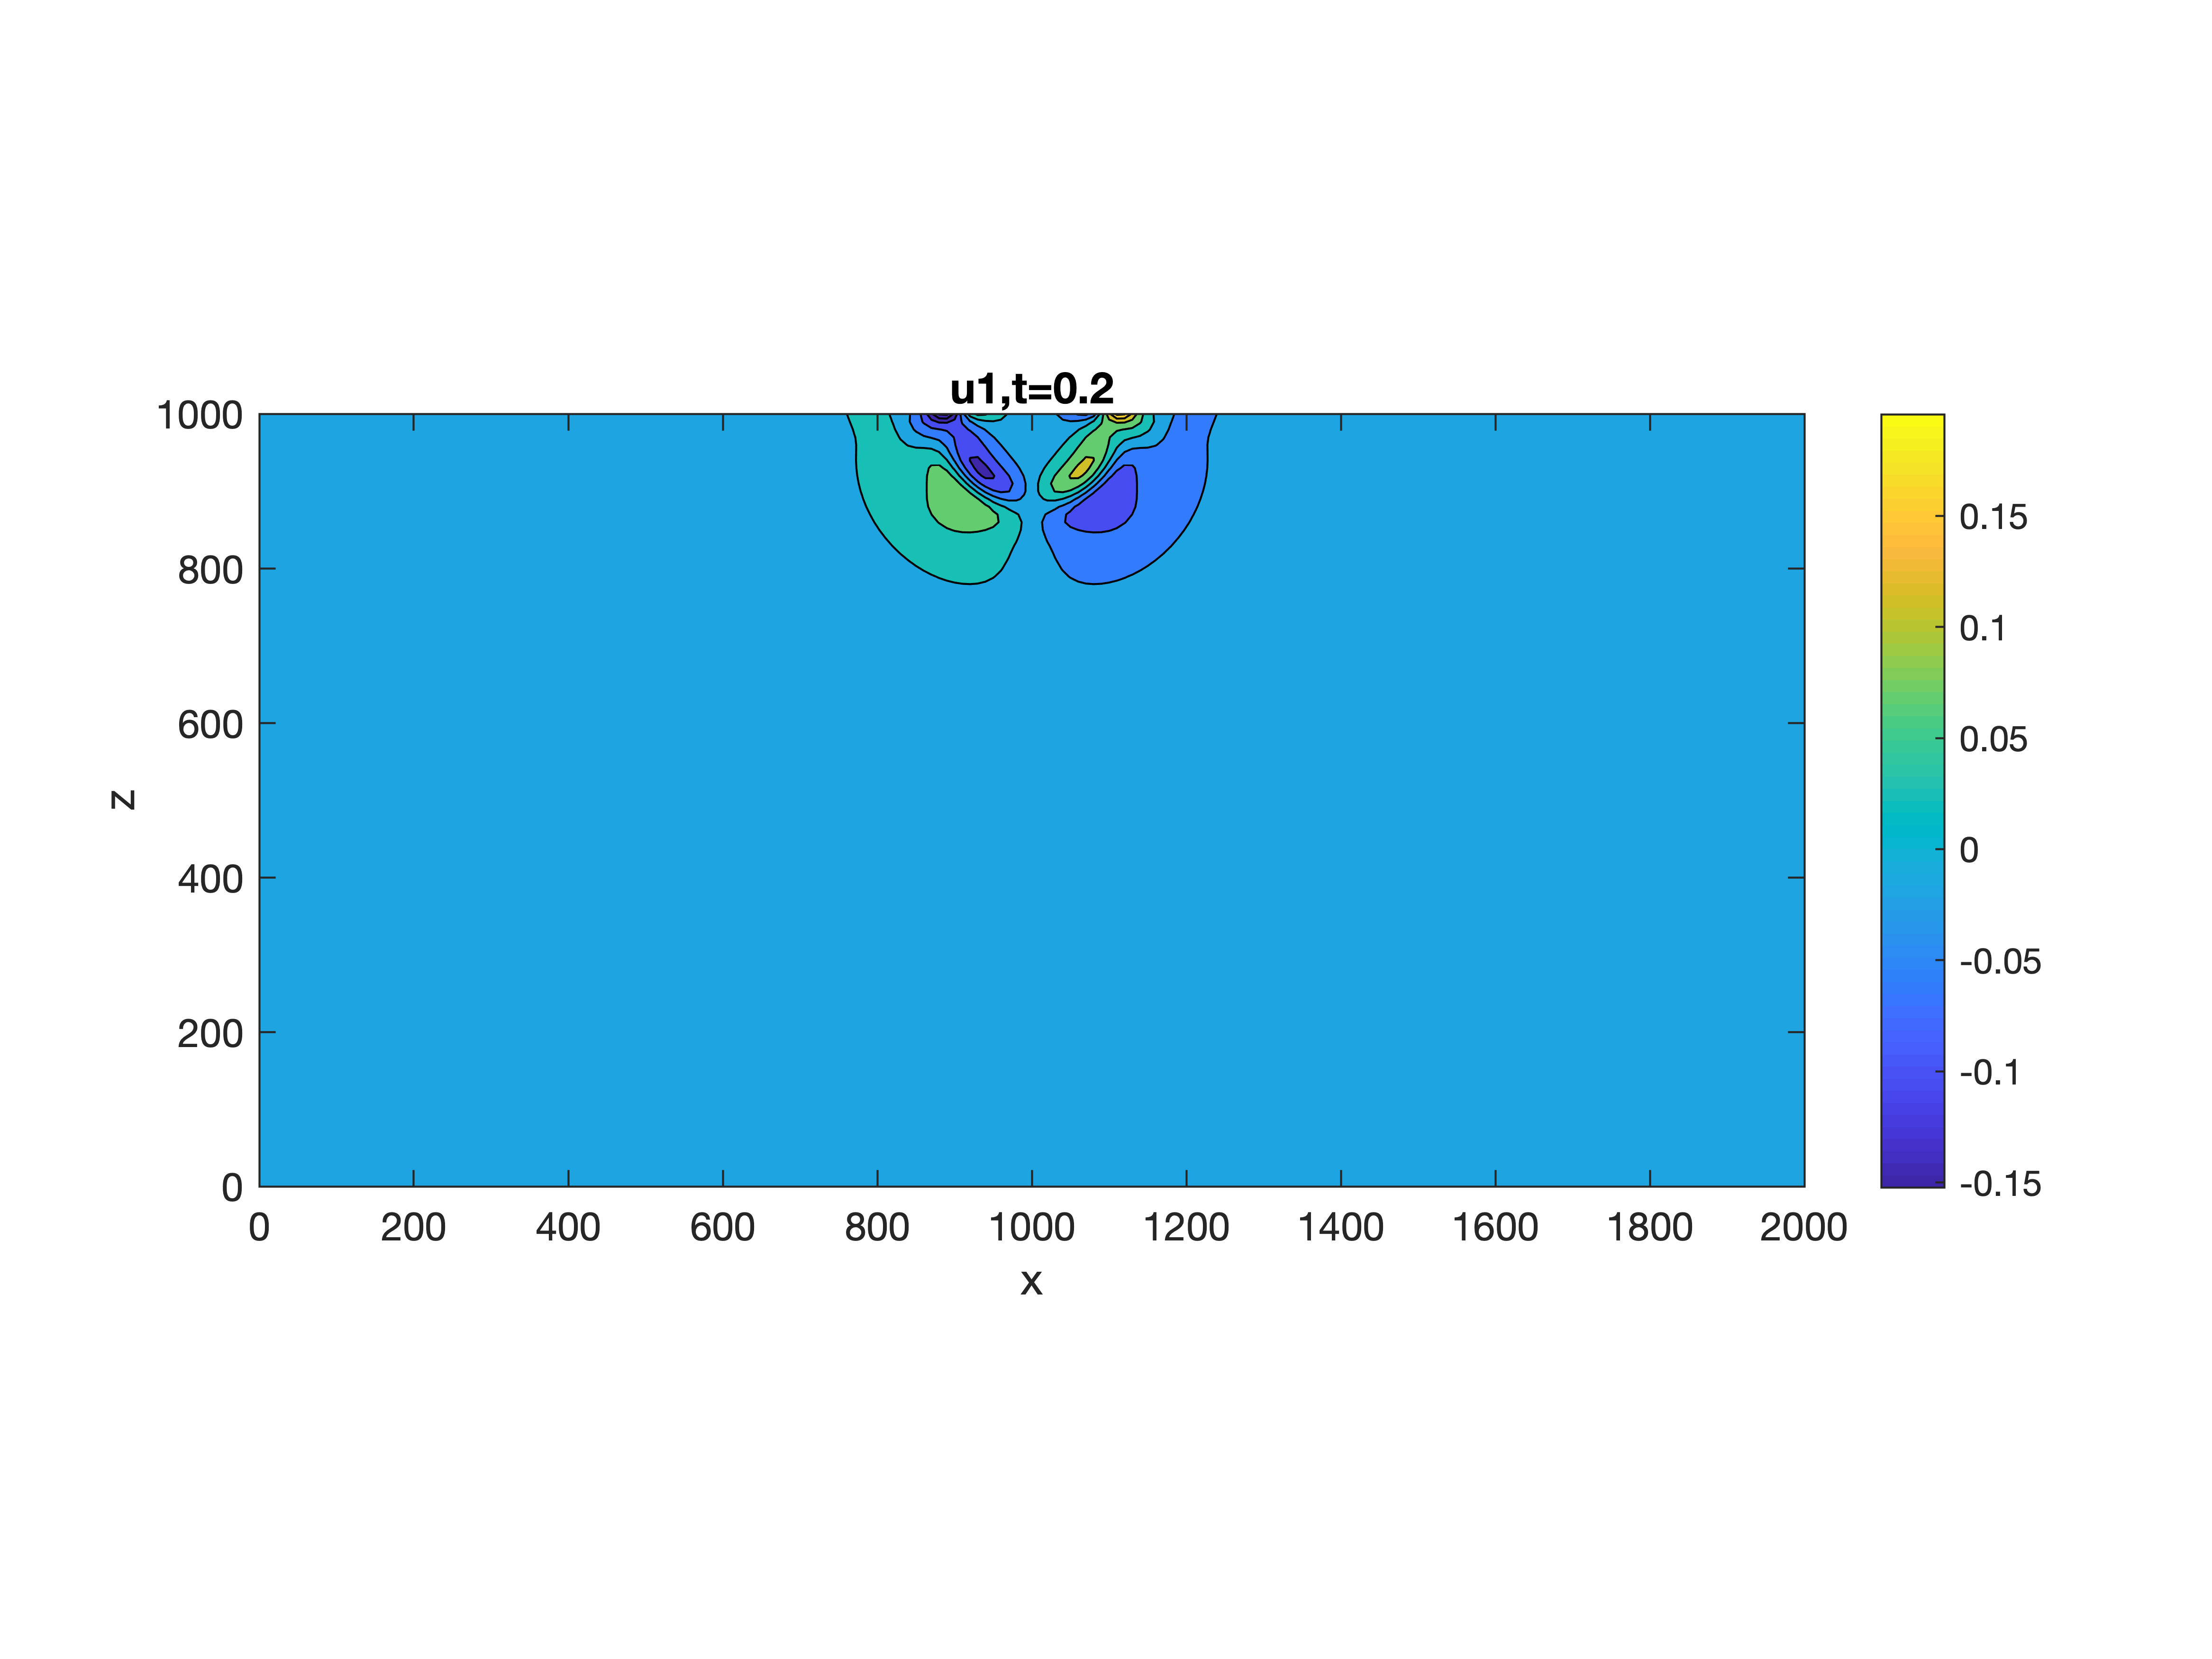
\includegraphics[width=0.4\textwidth,trim={0 2.8cm 0 2.8cm}, clip]{u1_t02_cartesian.png}
	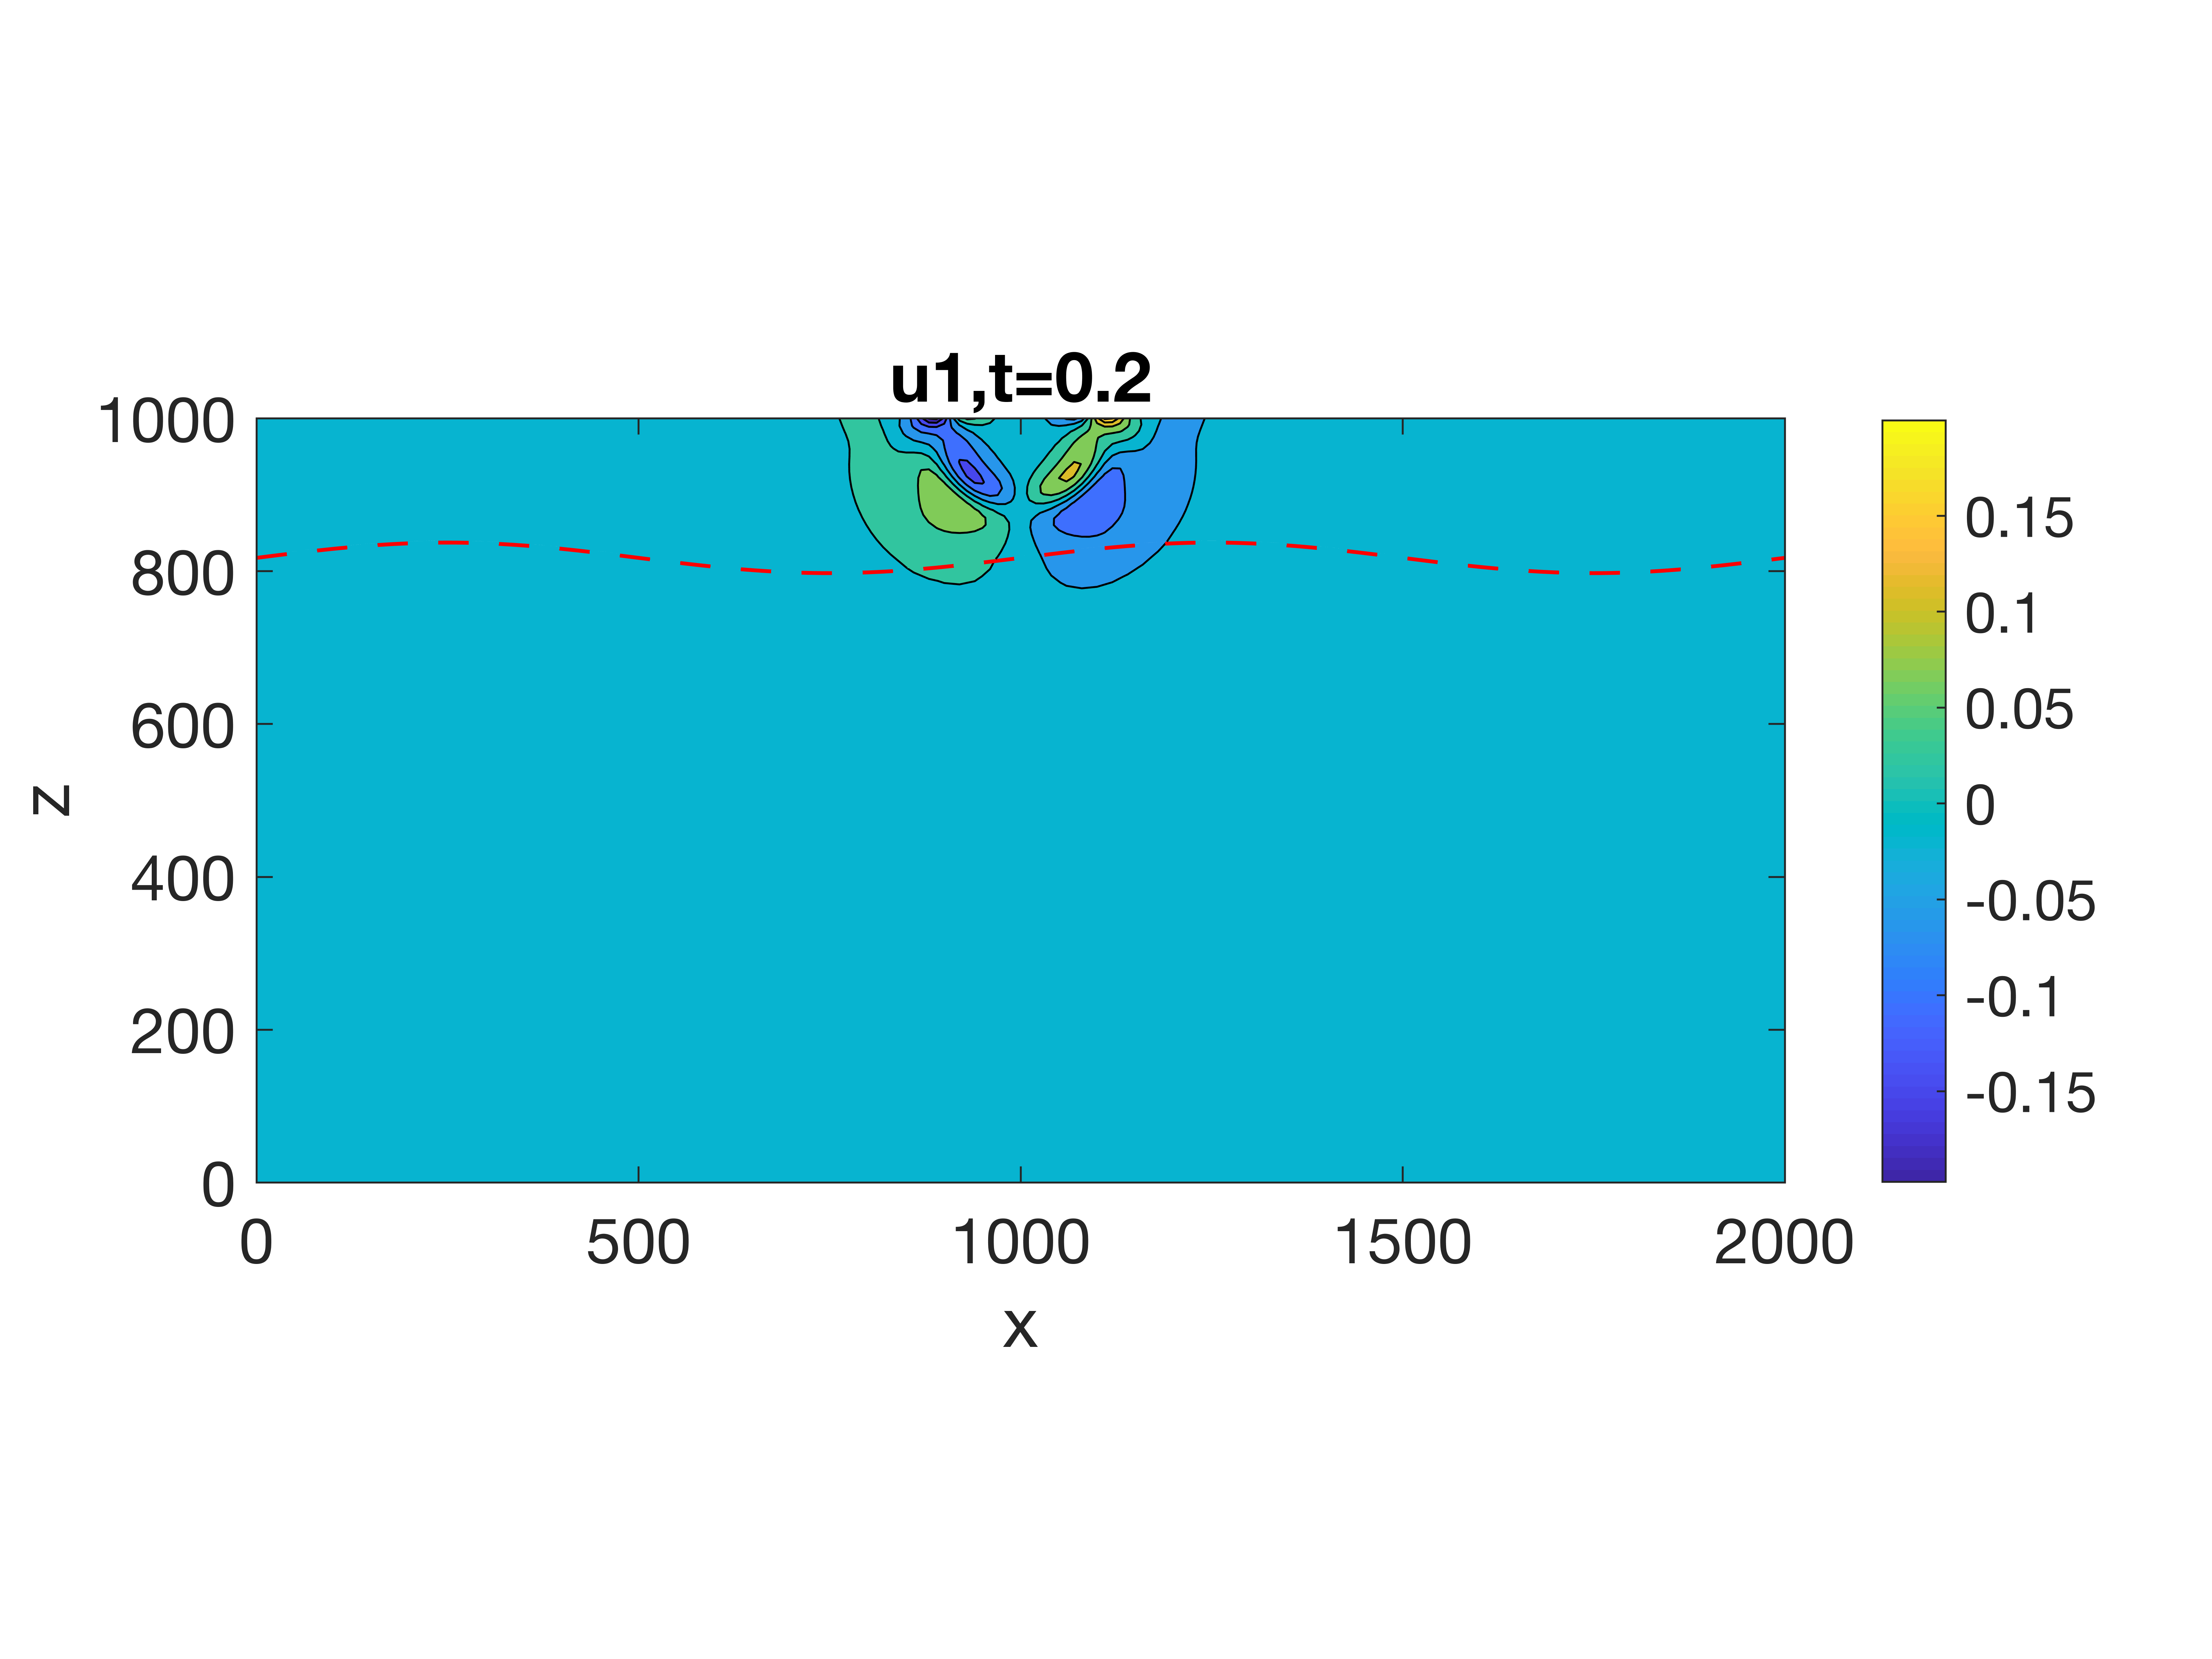
\includegraphics[width=0.4\textwidth,trim={0 2.8cm 0 2.8cm}, clip]{u1_t02_curvi_mr.png}\\
	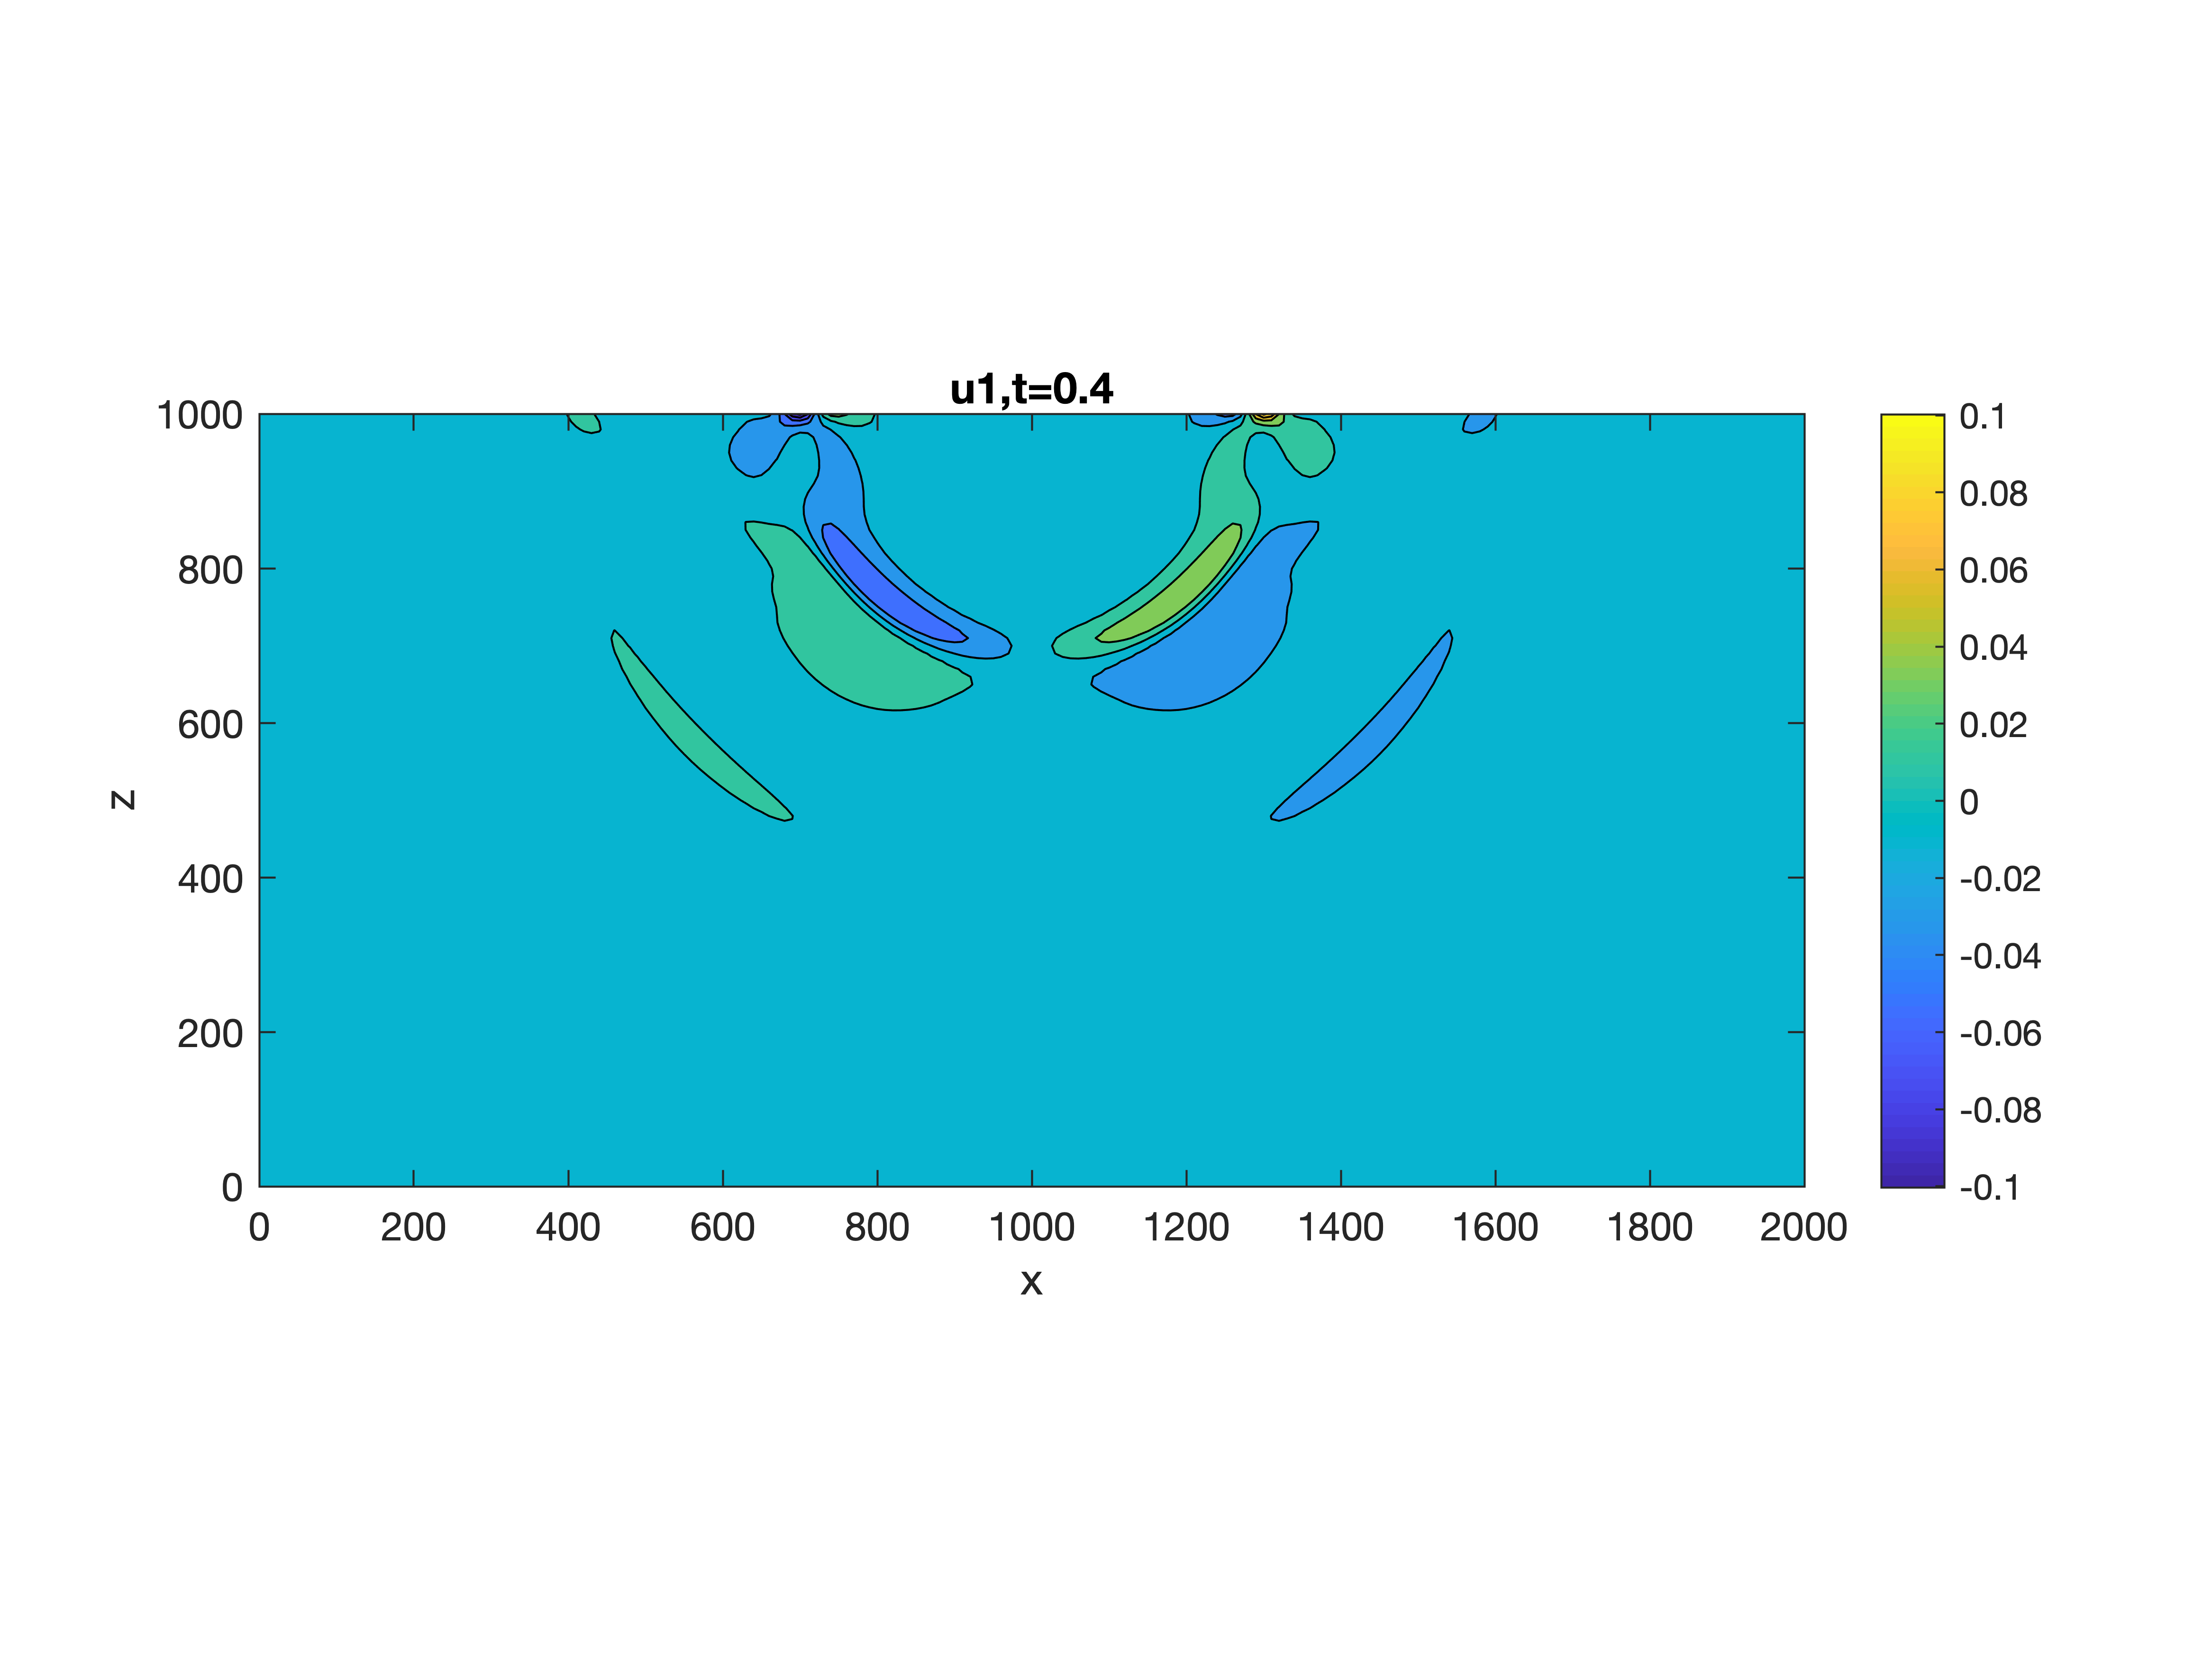
\includegraphics[width=0.4\textwidth,trim={0 2.8cm 0 2.8cm}, clip]{u1_t04_cartesian.png}
	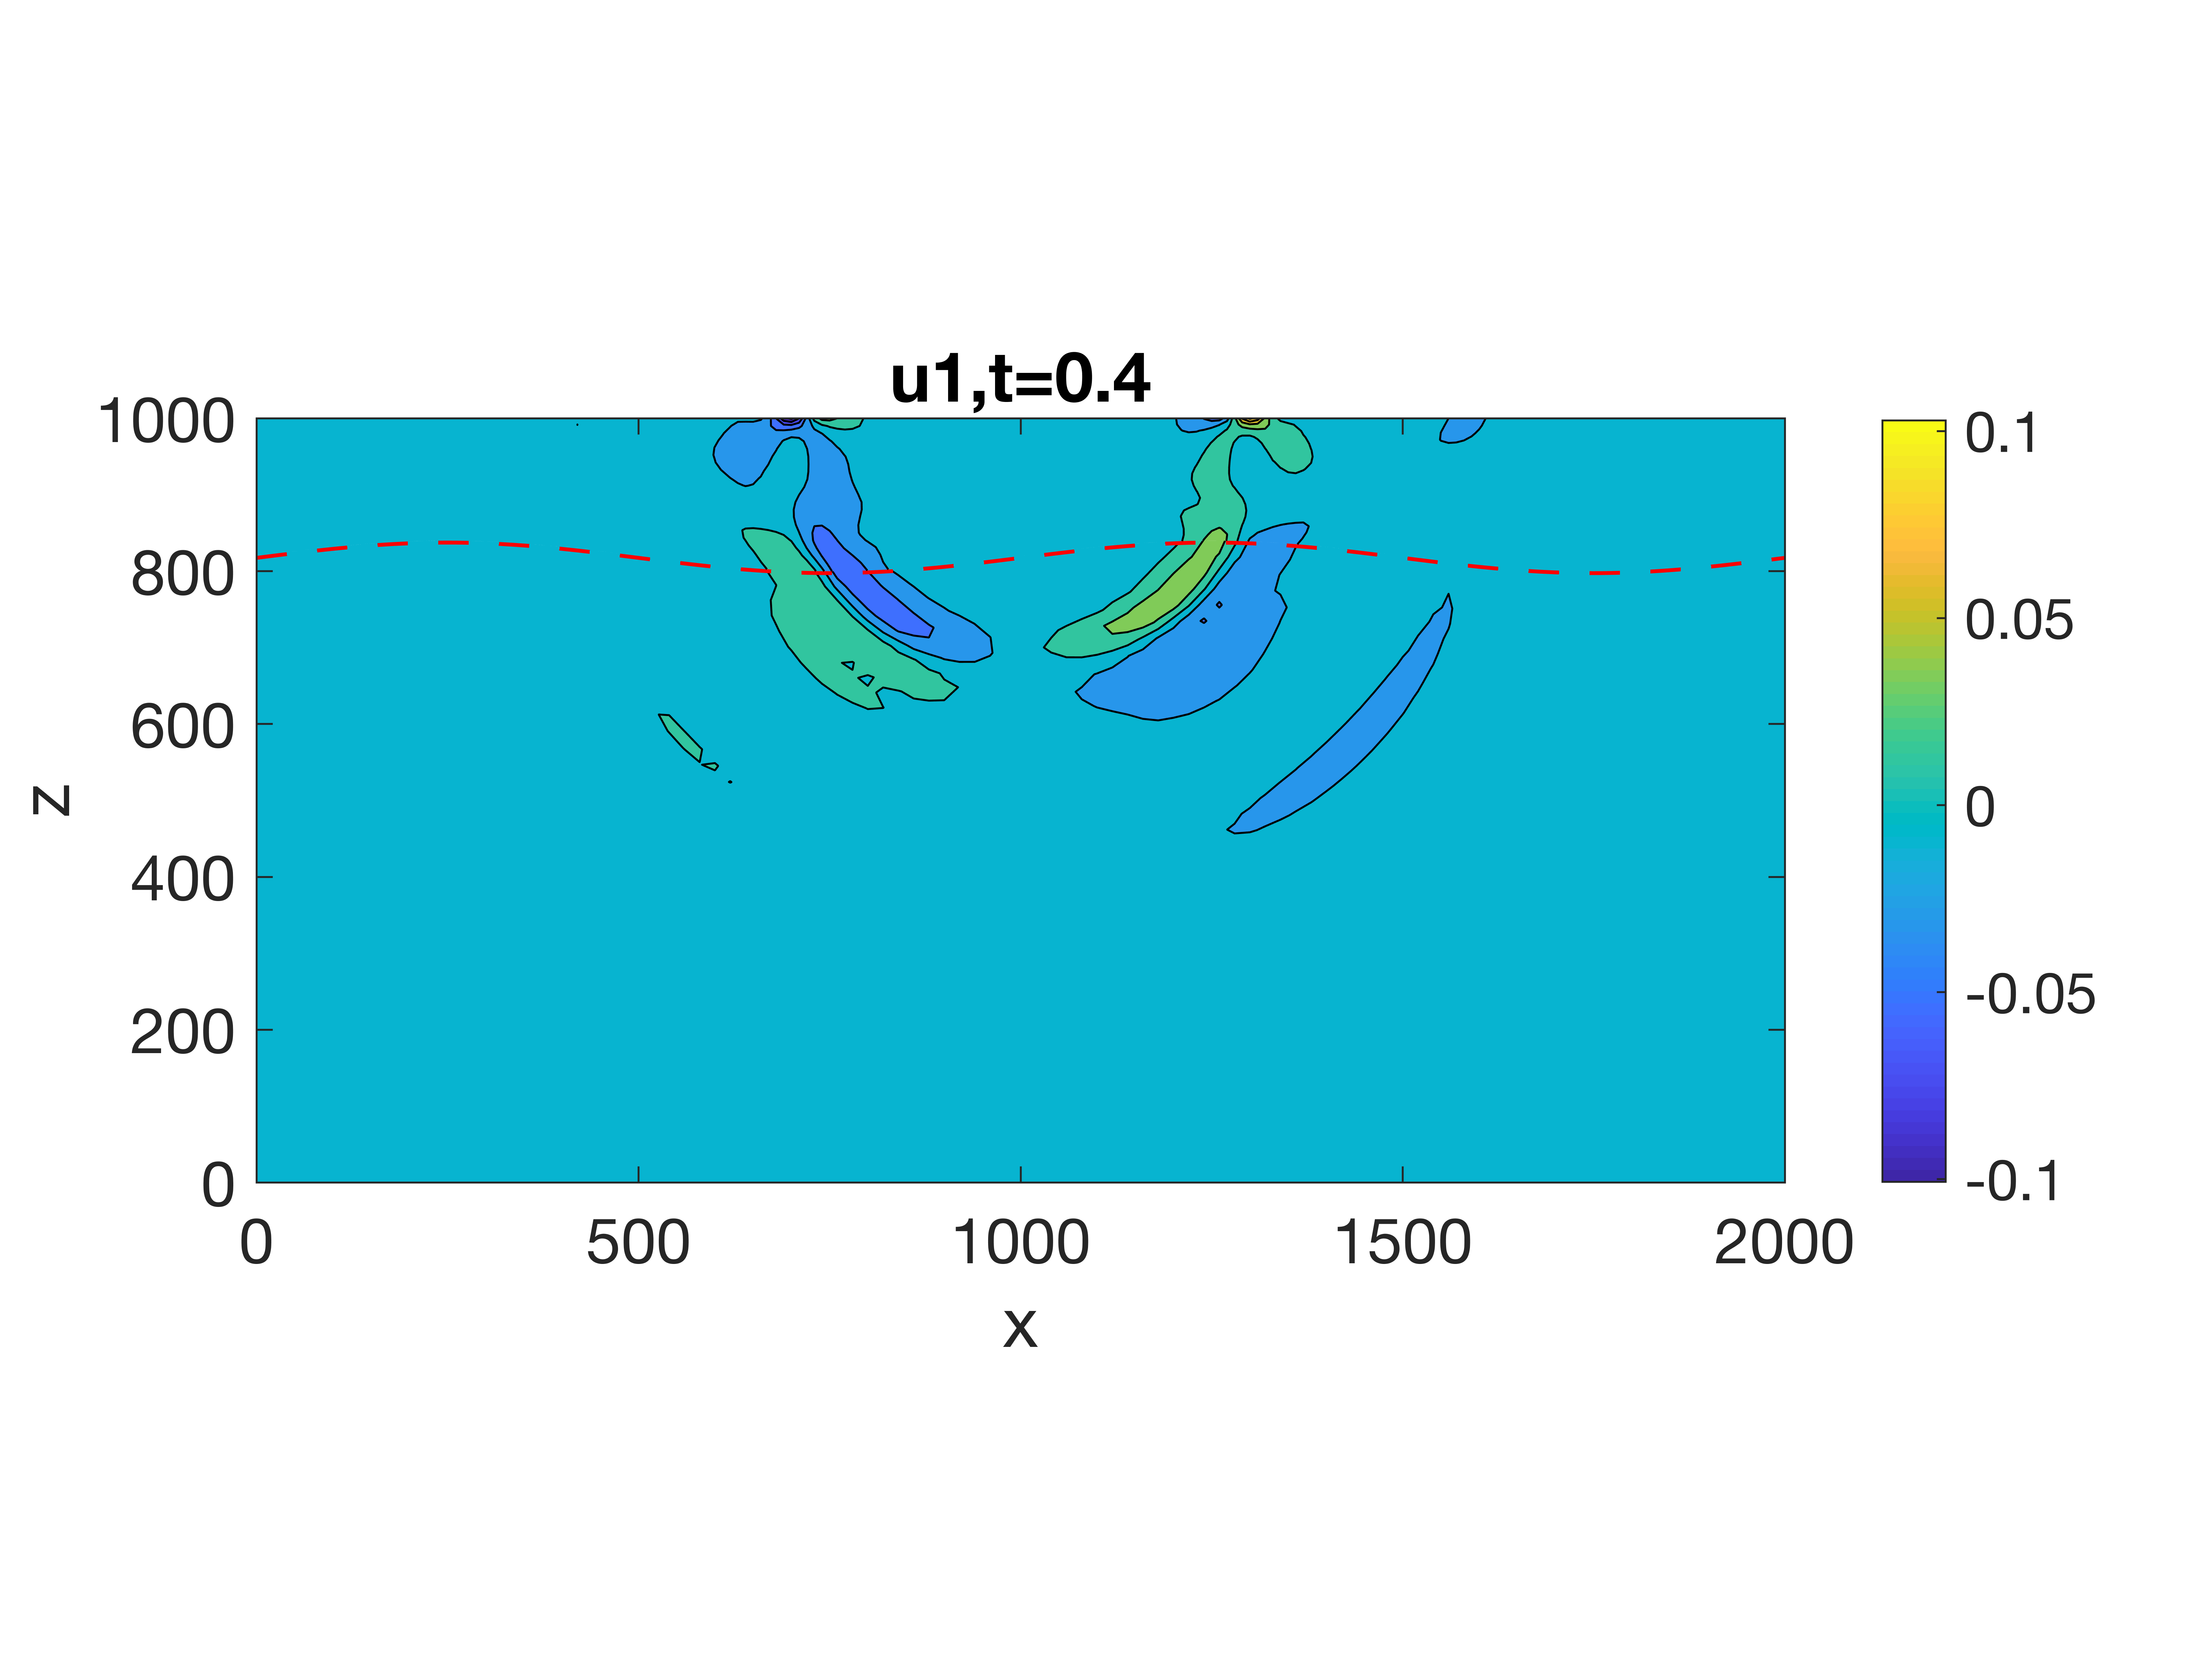
\includegraphics[width=0.4\textwidth,trim={0 2.8cm 0 2.8cm}, clip]{u1_t04_curvi_mr.png}
	\caption{The graph for $u_1$. From left to right are for Cartesian mesh without mesh refinement interface and curvi-linear mesh with mesh refinement interface respectively. From top to bottom are for $t = 0.2$ and $t = 0.4$ respectively.}\label{u1}
\end{figure}

\begin{figure}[htbp]
	\centering
	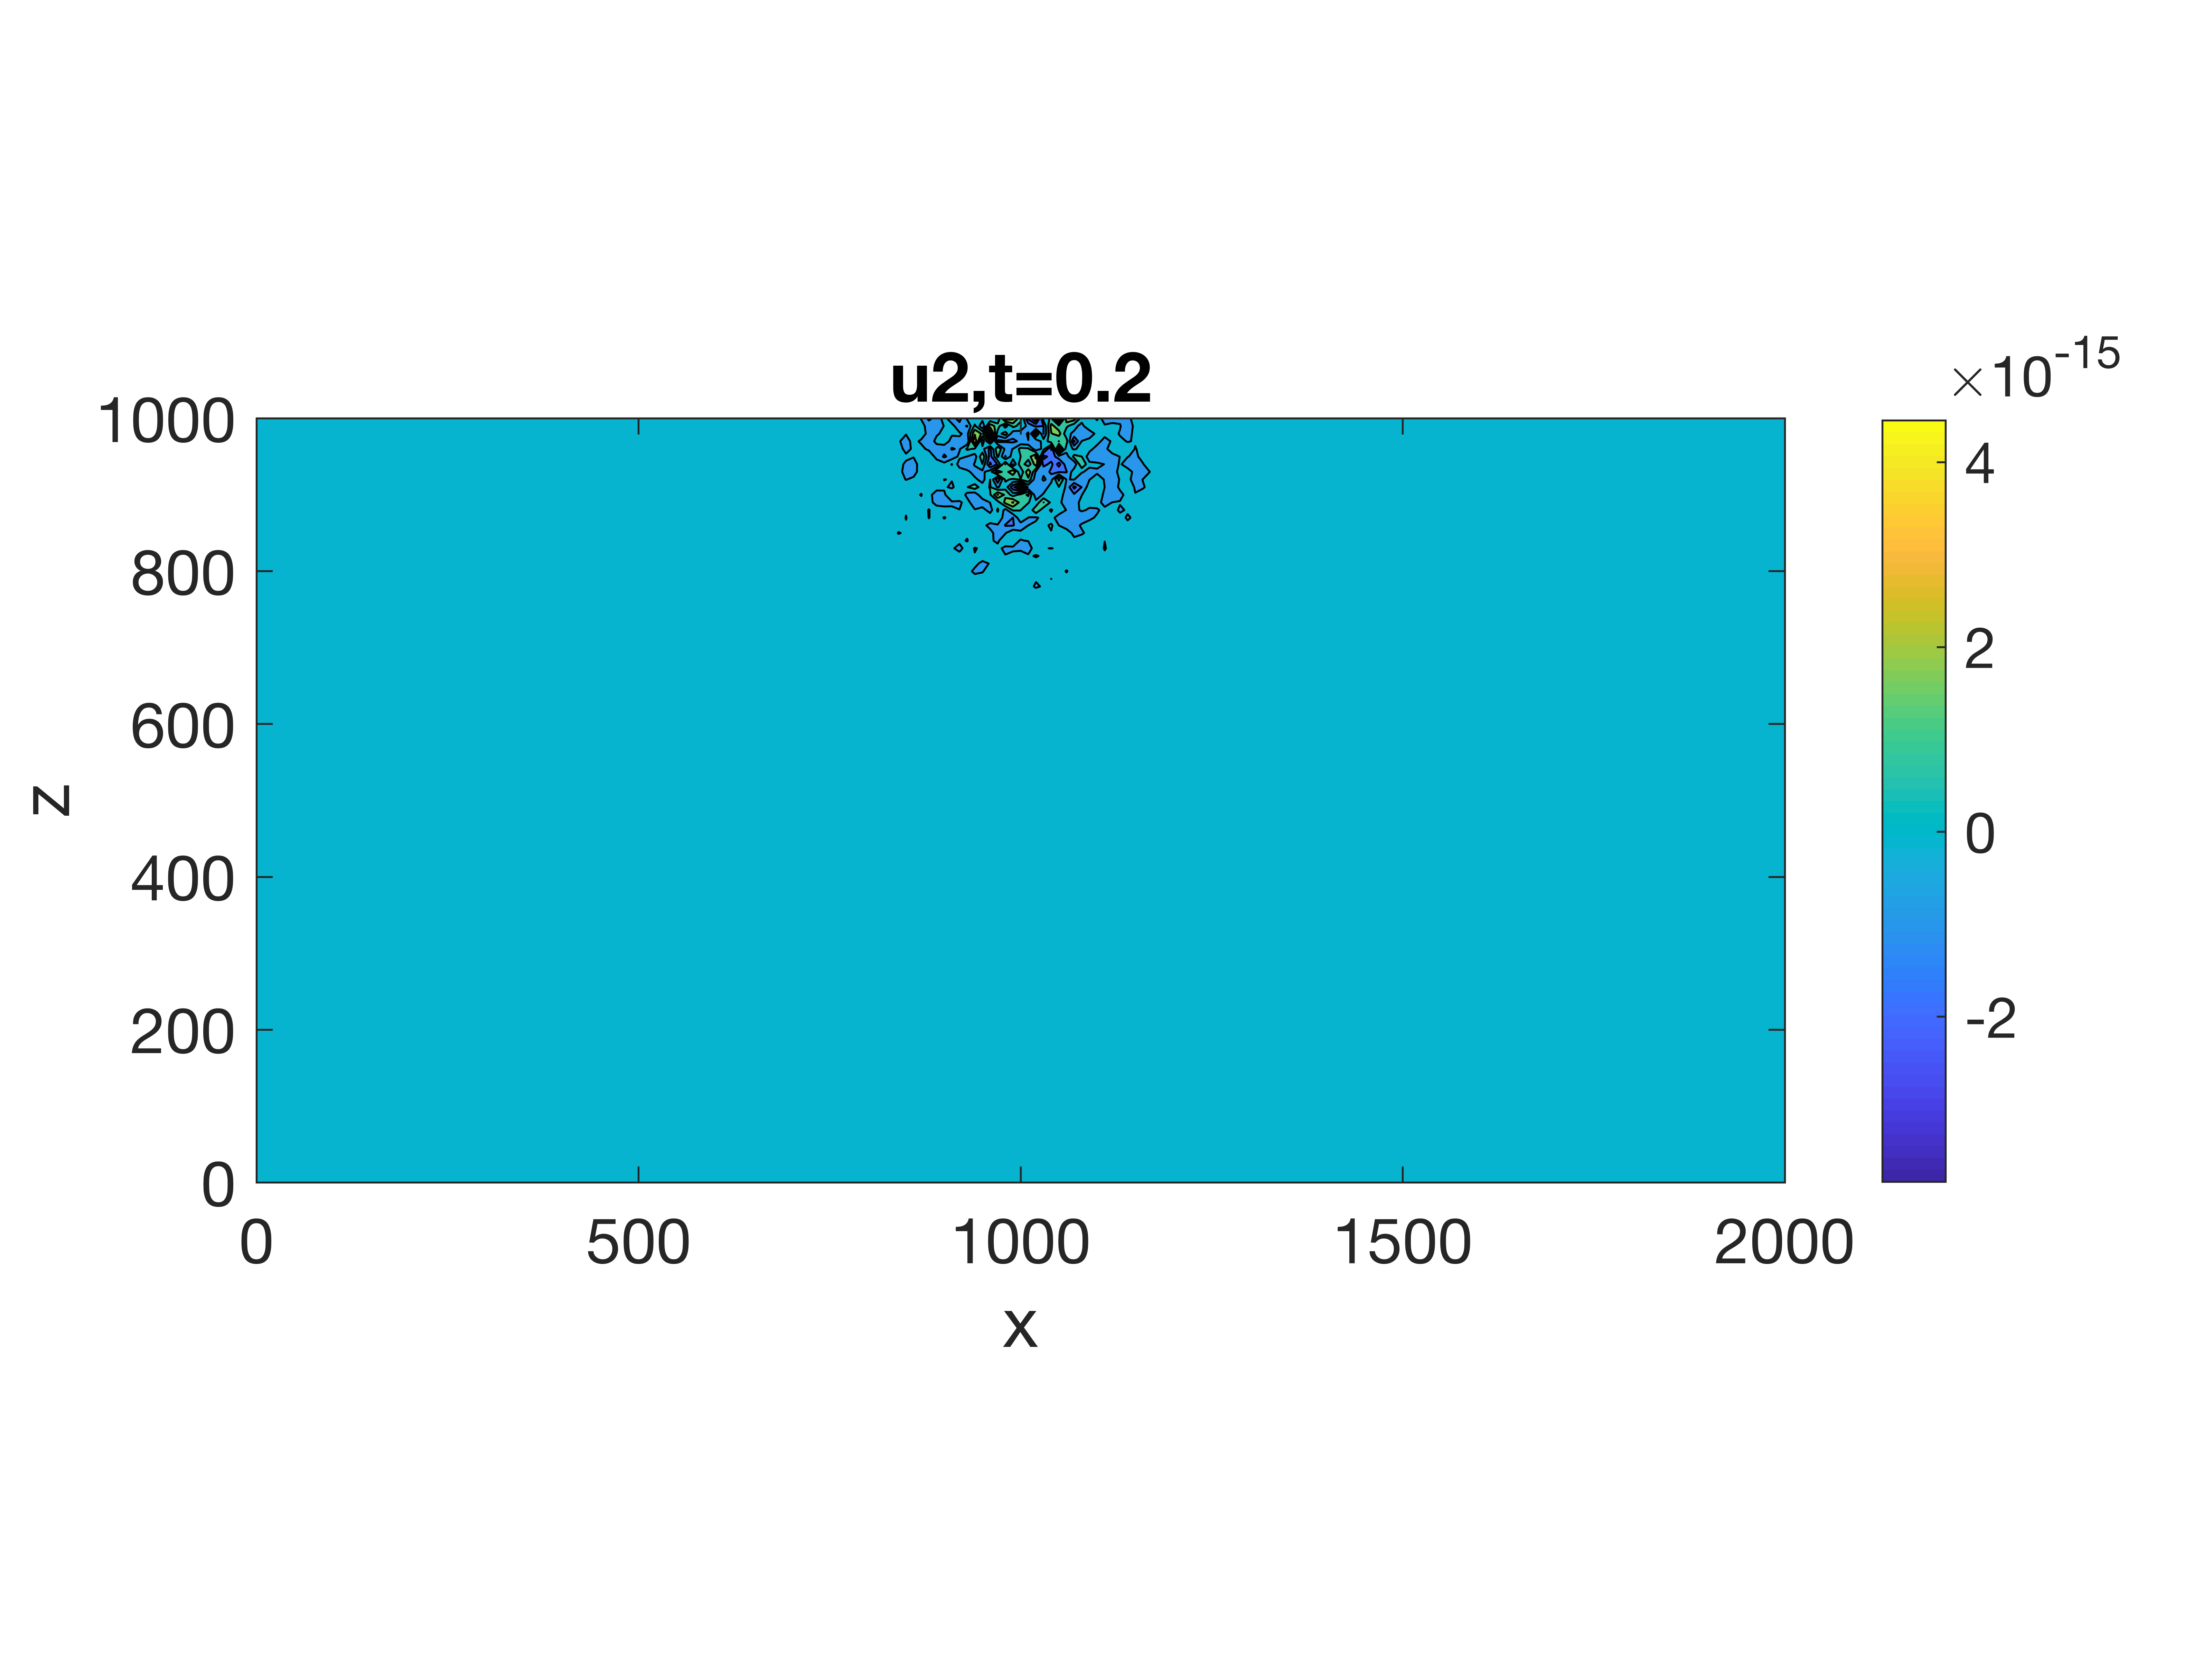
\includegraphics[width=0.4\textwidth,trim={0 2.8cm 0 2.8cm}, clip]{u2_t02_cartesian.png}
	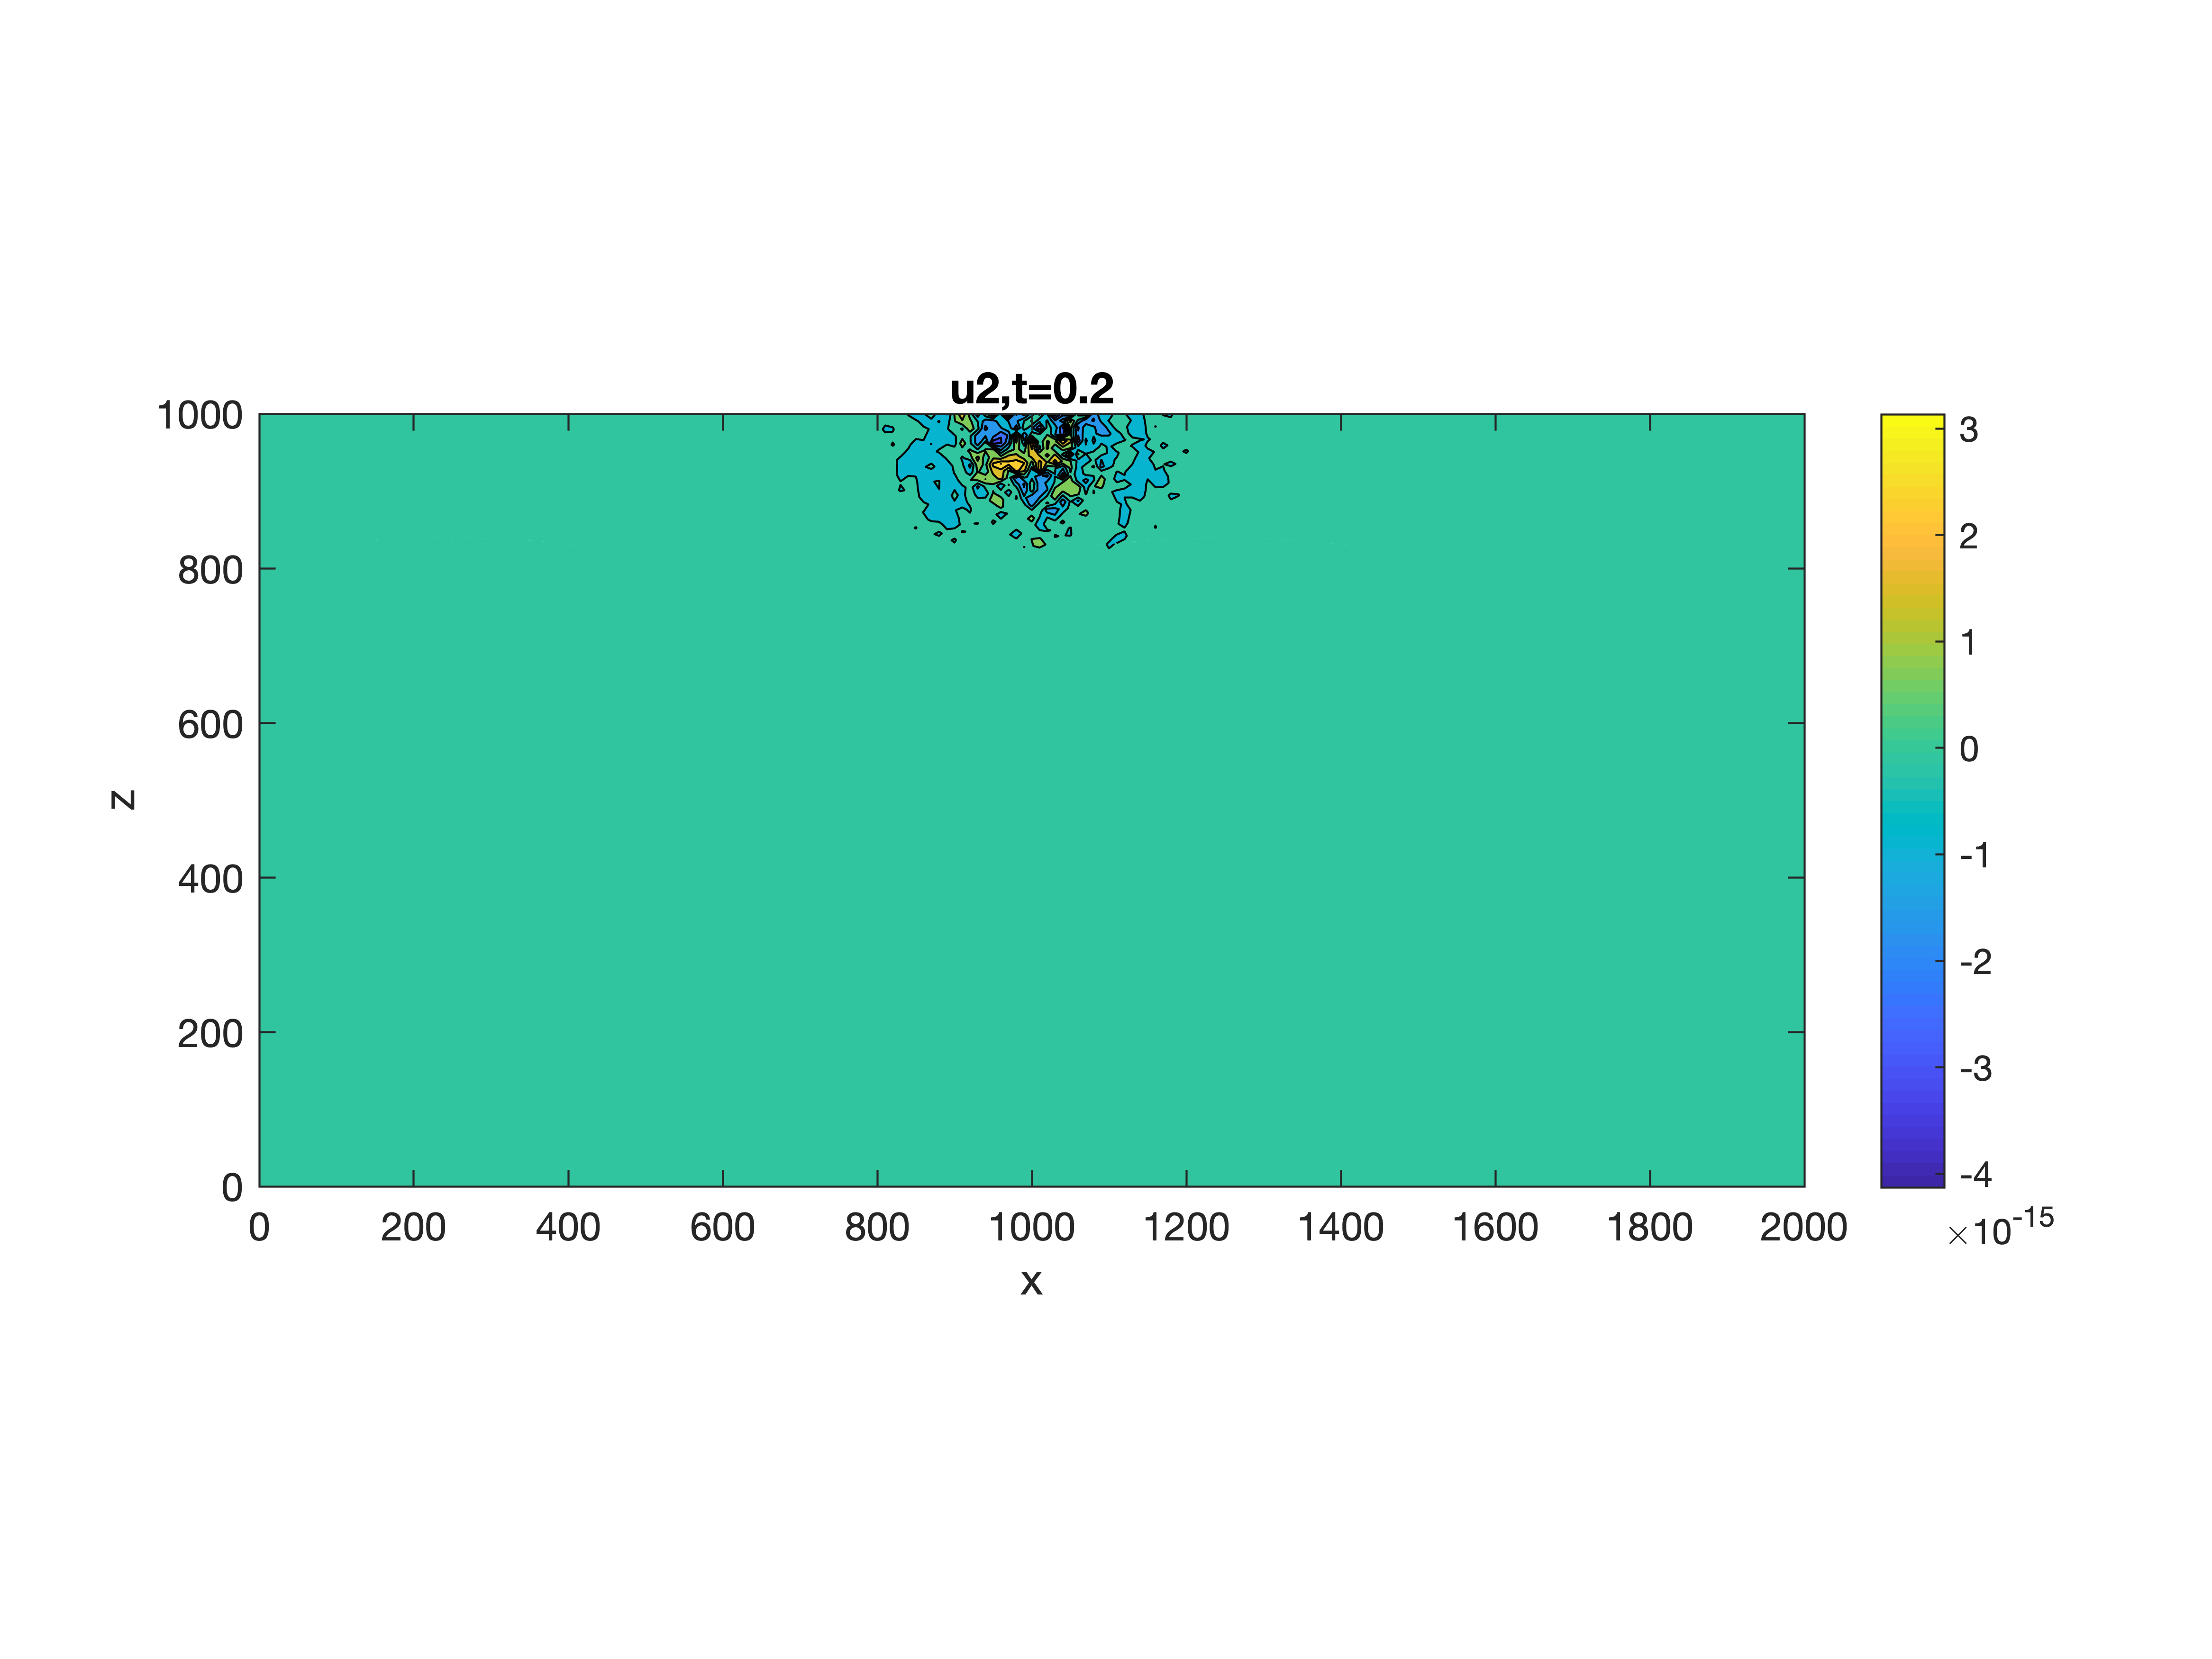
\includegraphics[width=0.4\textwidth,trim={0 2.8cm 0 2.8cm}, clip]{u2_t02_curvi_mr.png}\\
	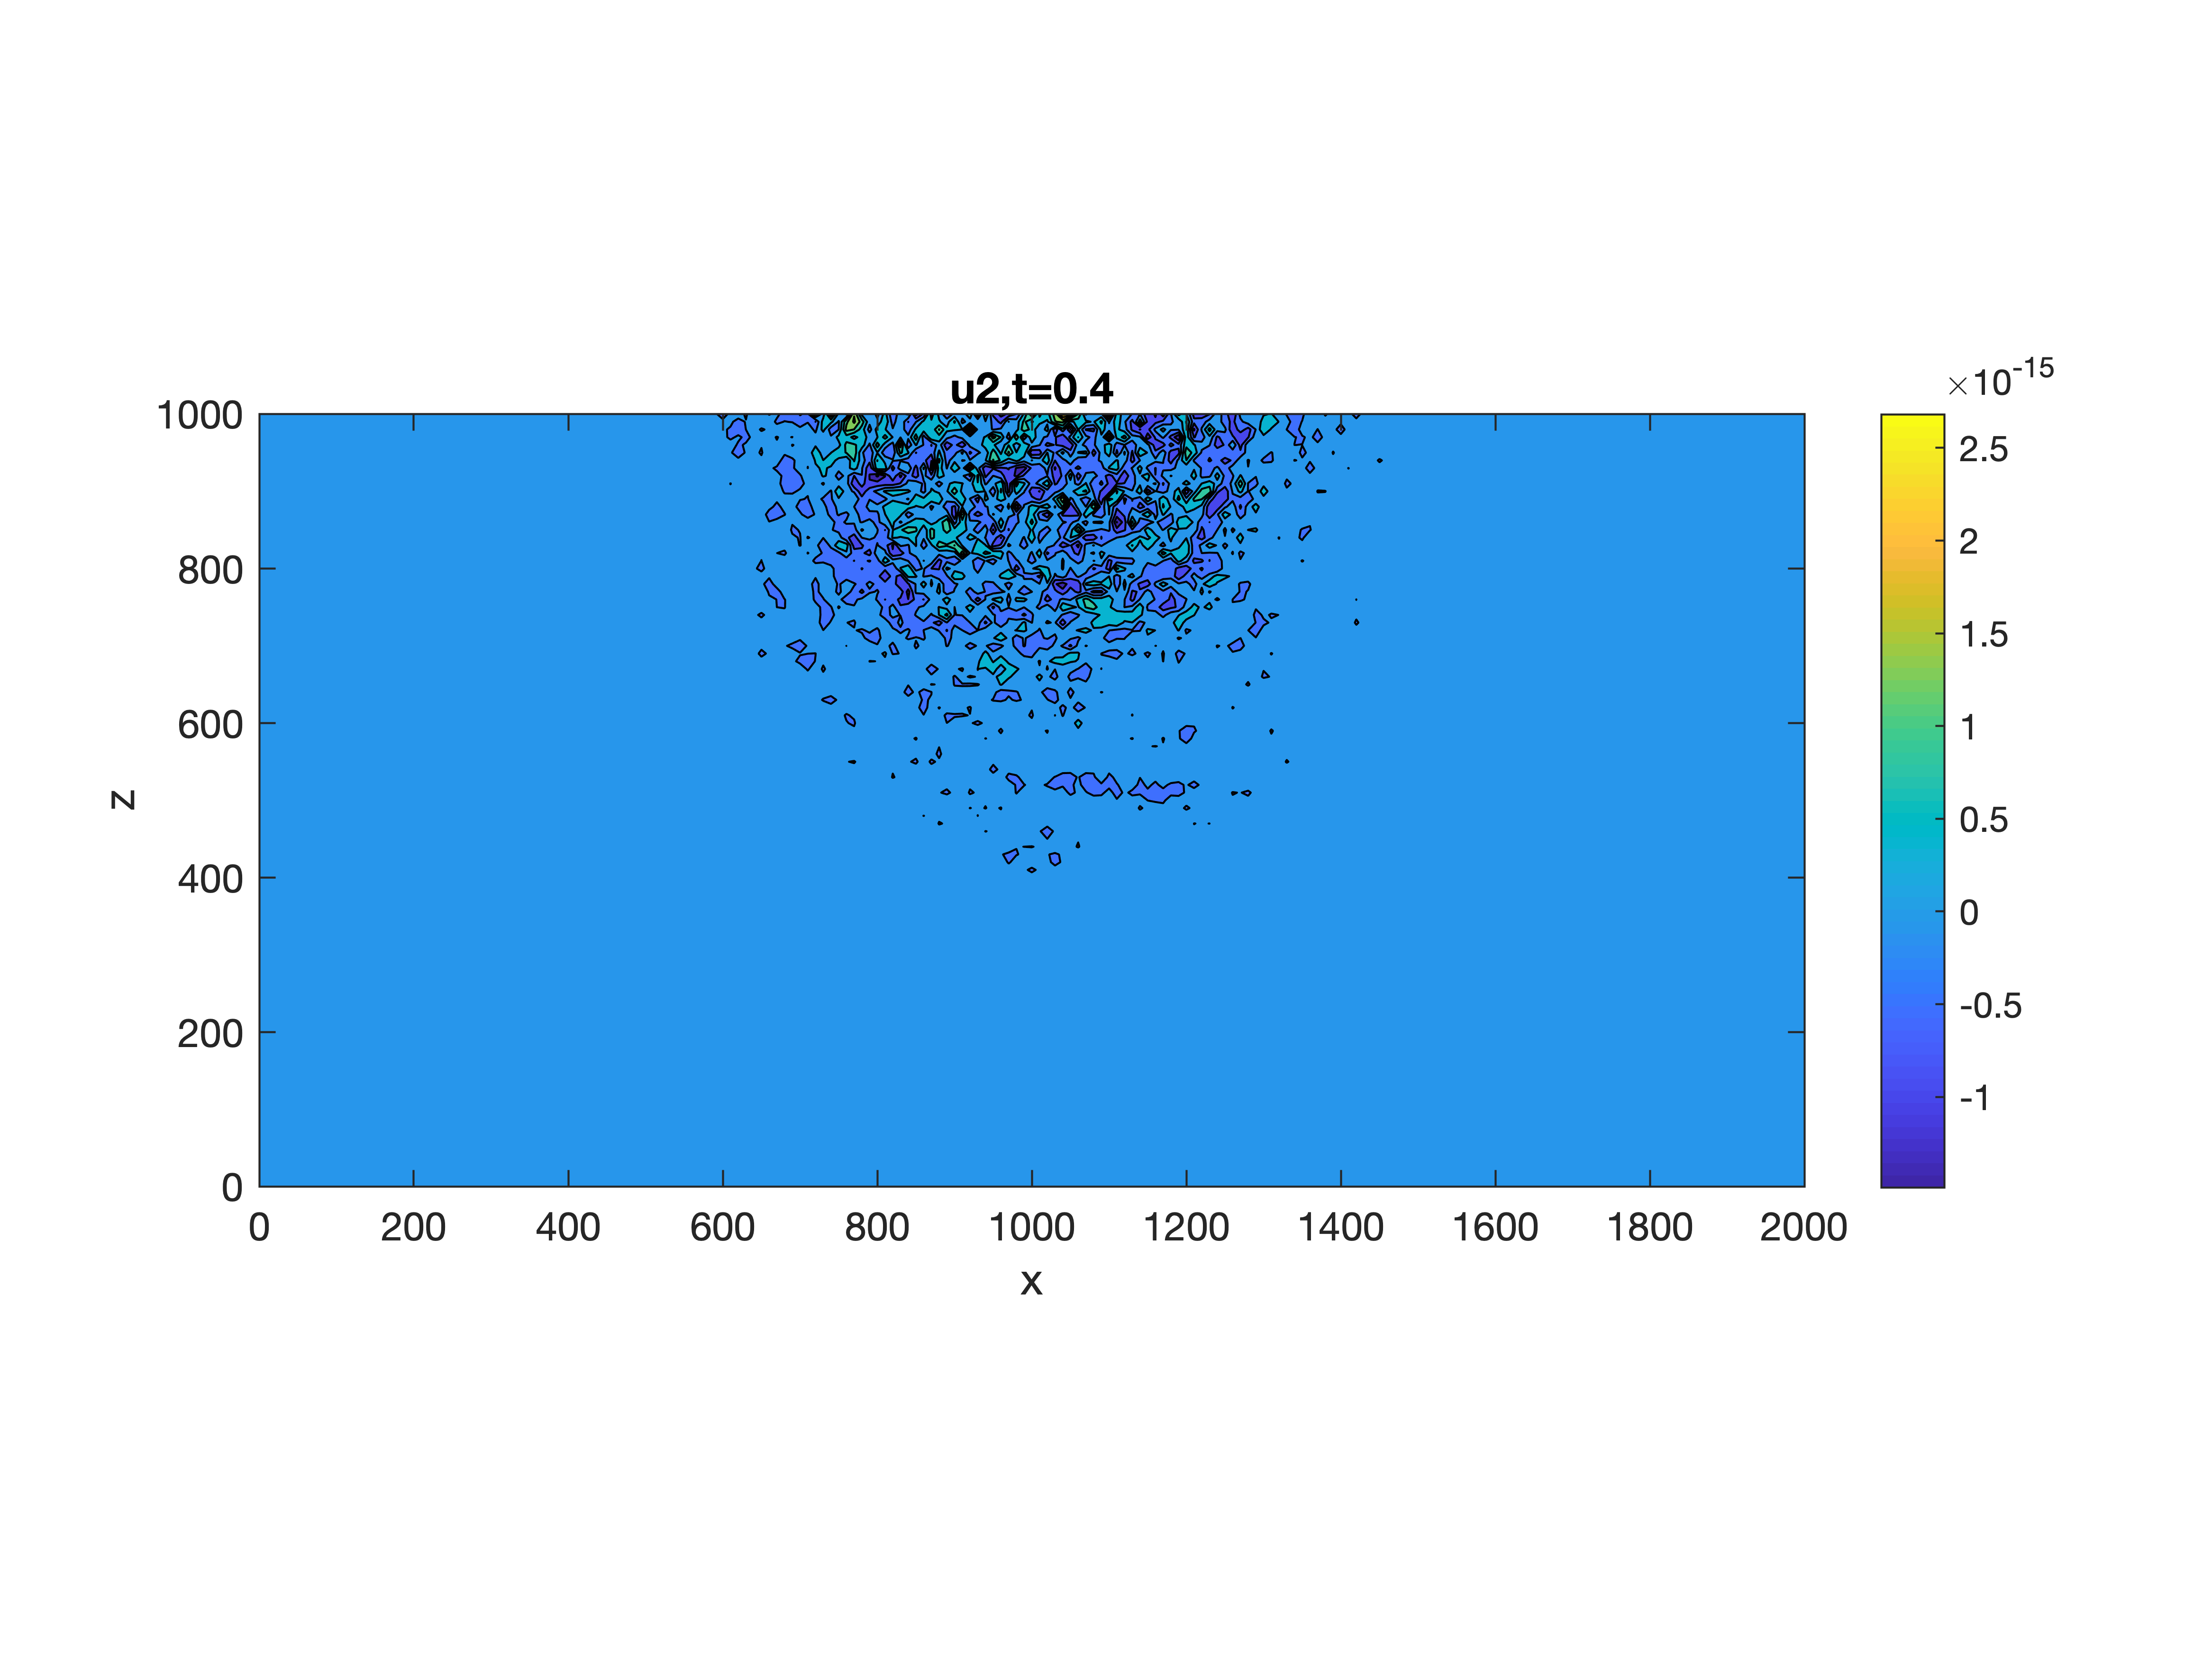
\includegraphics[width=0.4\textwidth,trim={0 2.8cm 0 2.8cm}, clip]{u2_t04_cartesian.png}
	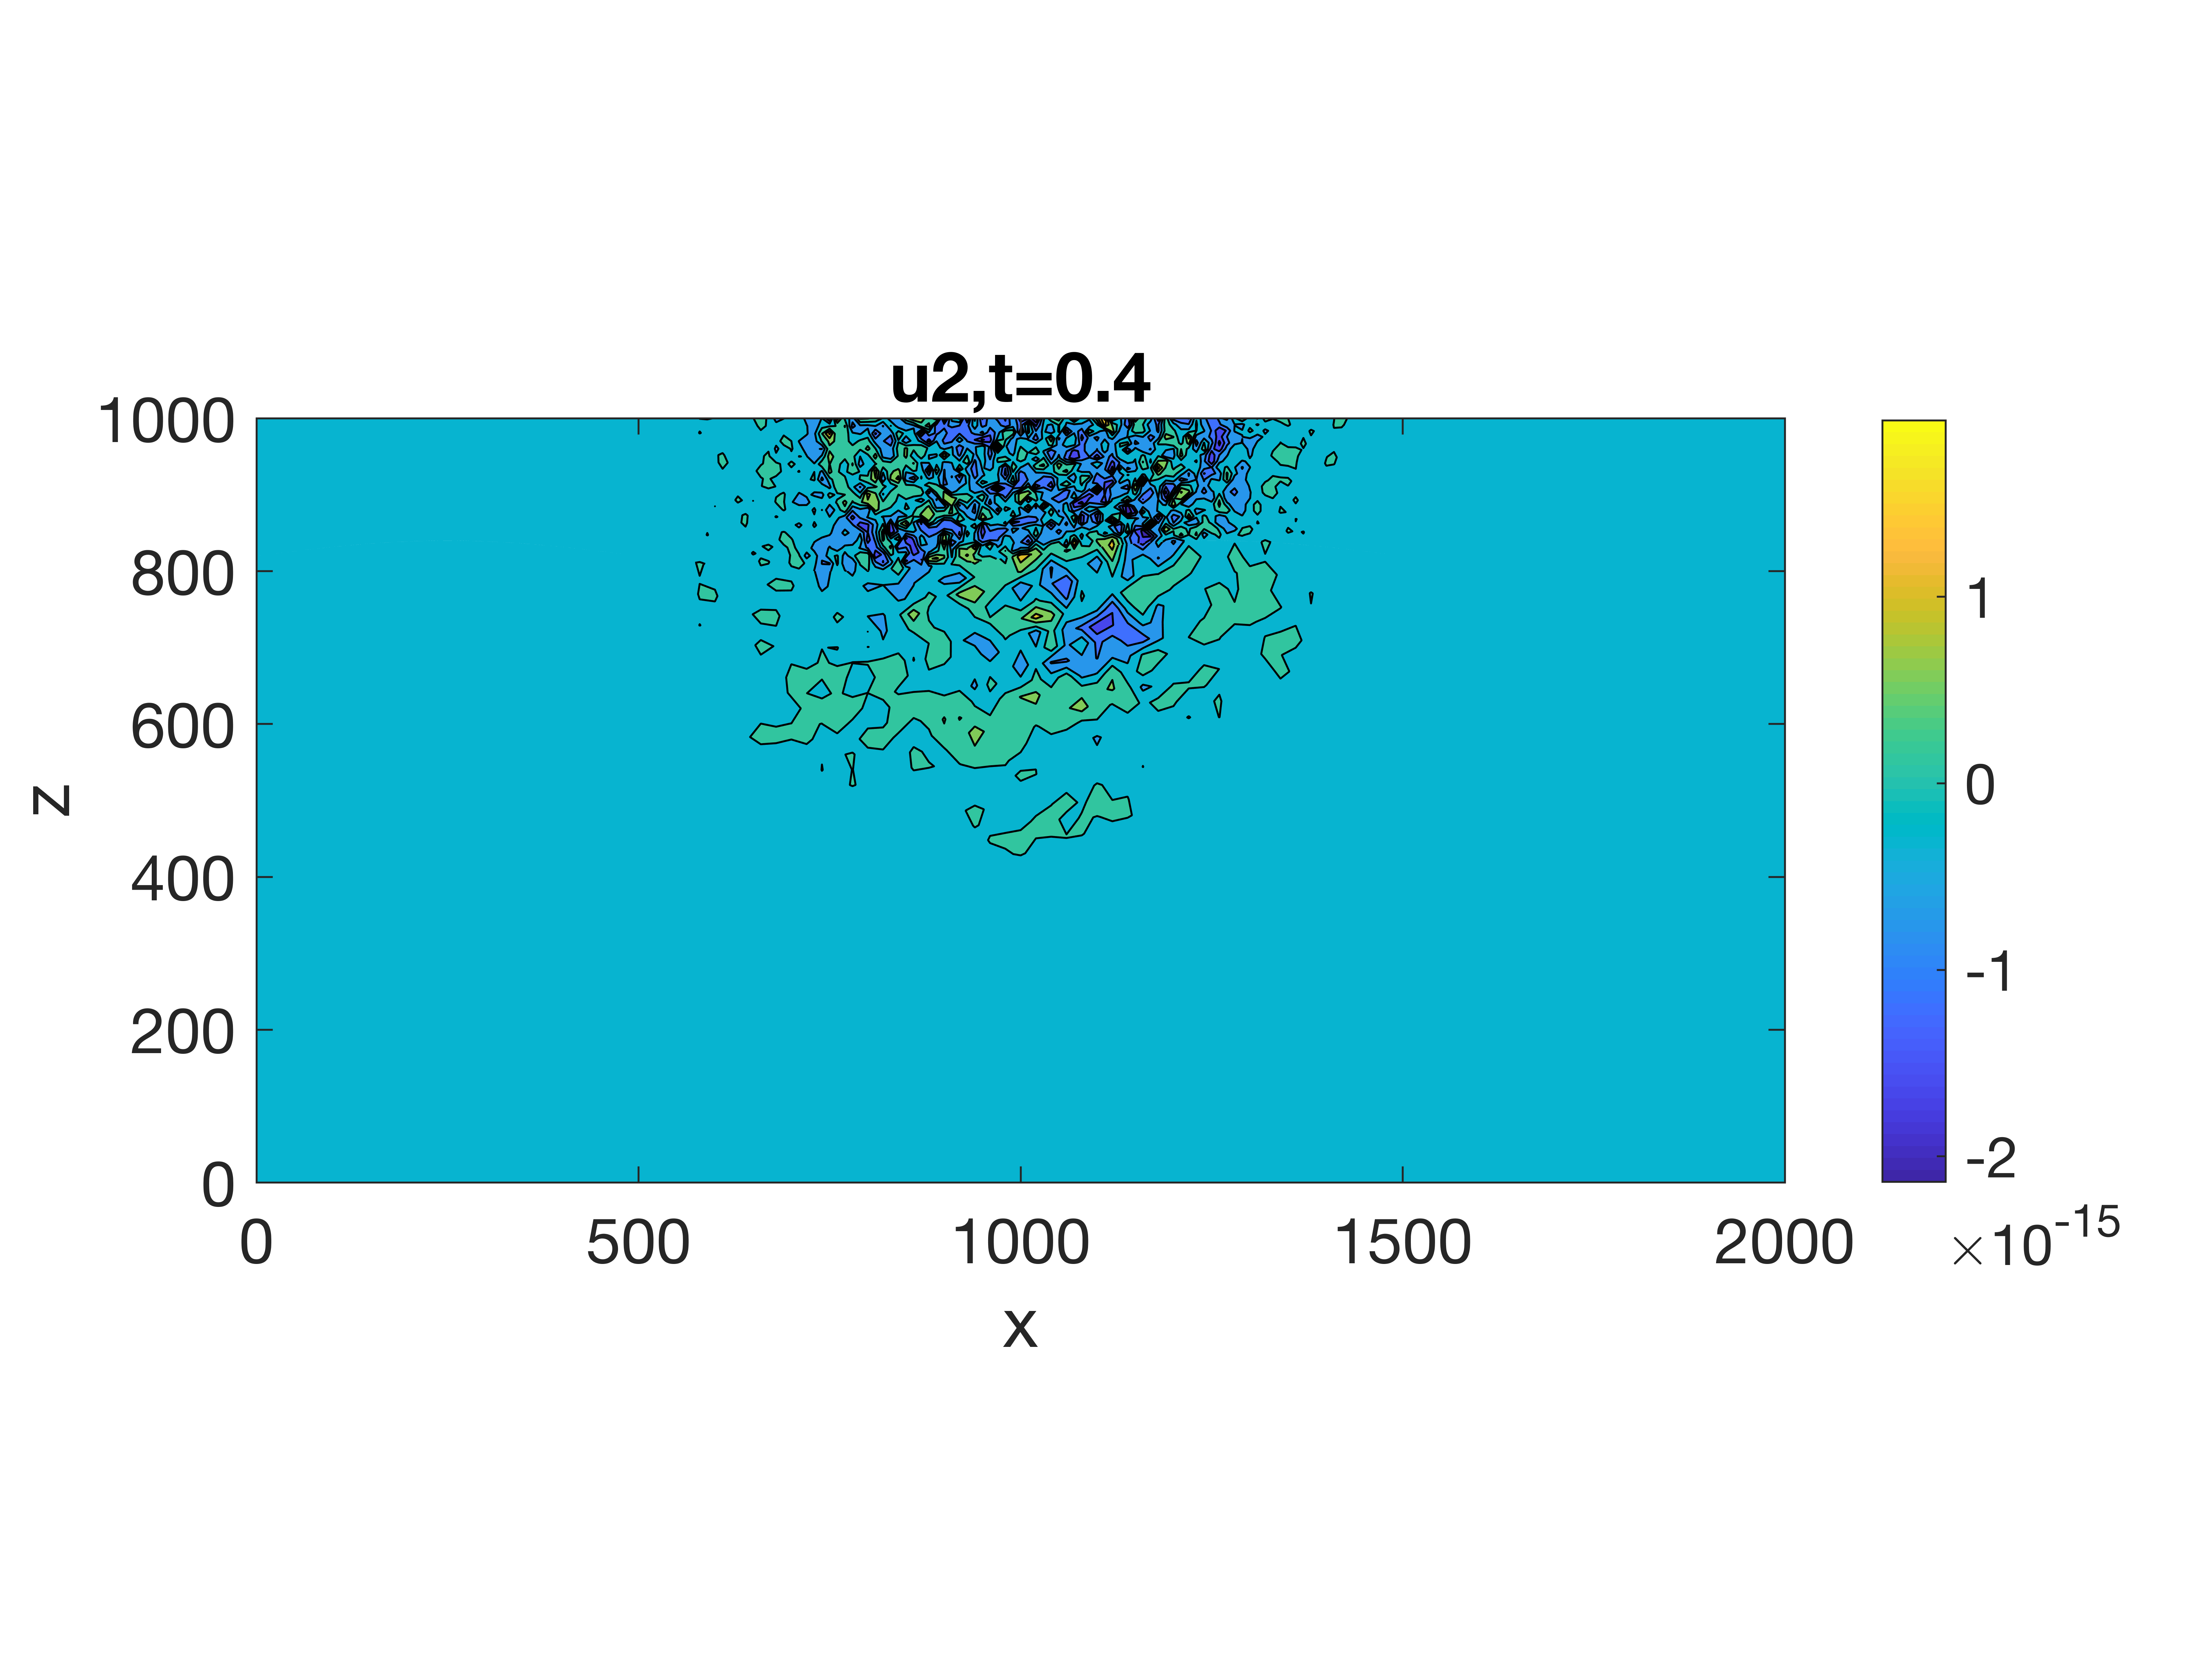
\includegraphics[width=0.4\textwidth,trim={0 2.8cm 0 2.8cm}, clip]{u2_t04_curvi_mr.png}
	\caption{The graph for $u_2$. From left to right are for Cartesian mesh without mesh refinement interface and curvi-linear mesh with mesh refinement interface respectively. From top to bottom are for $t = 0.2$ and $t = 0.4$ respectively.}\label{u2}
\end{figure}

\begin{figure}[htbp]
	\centering
	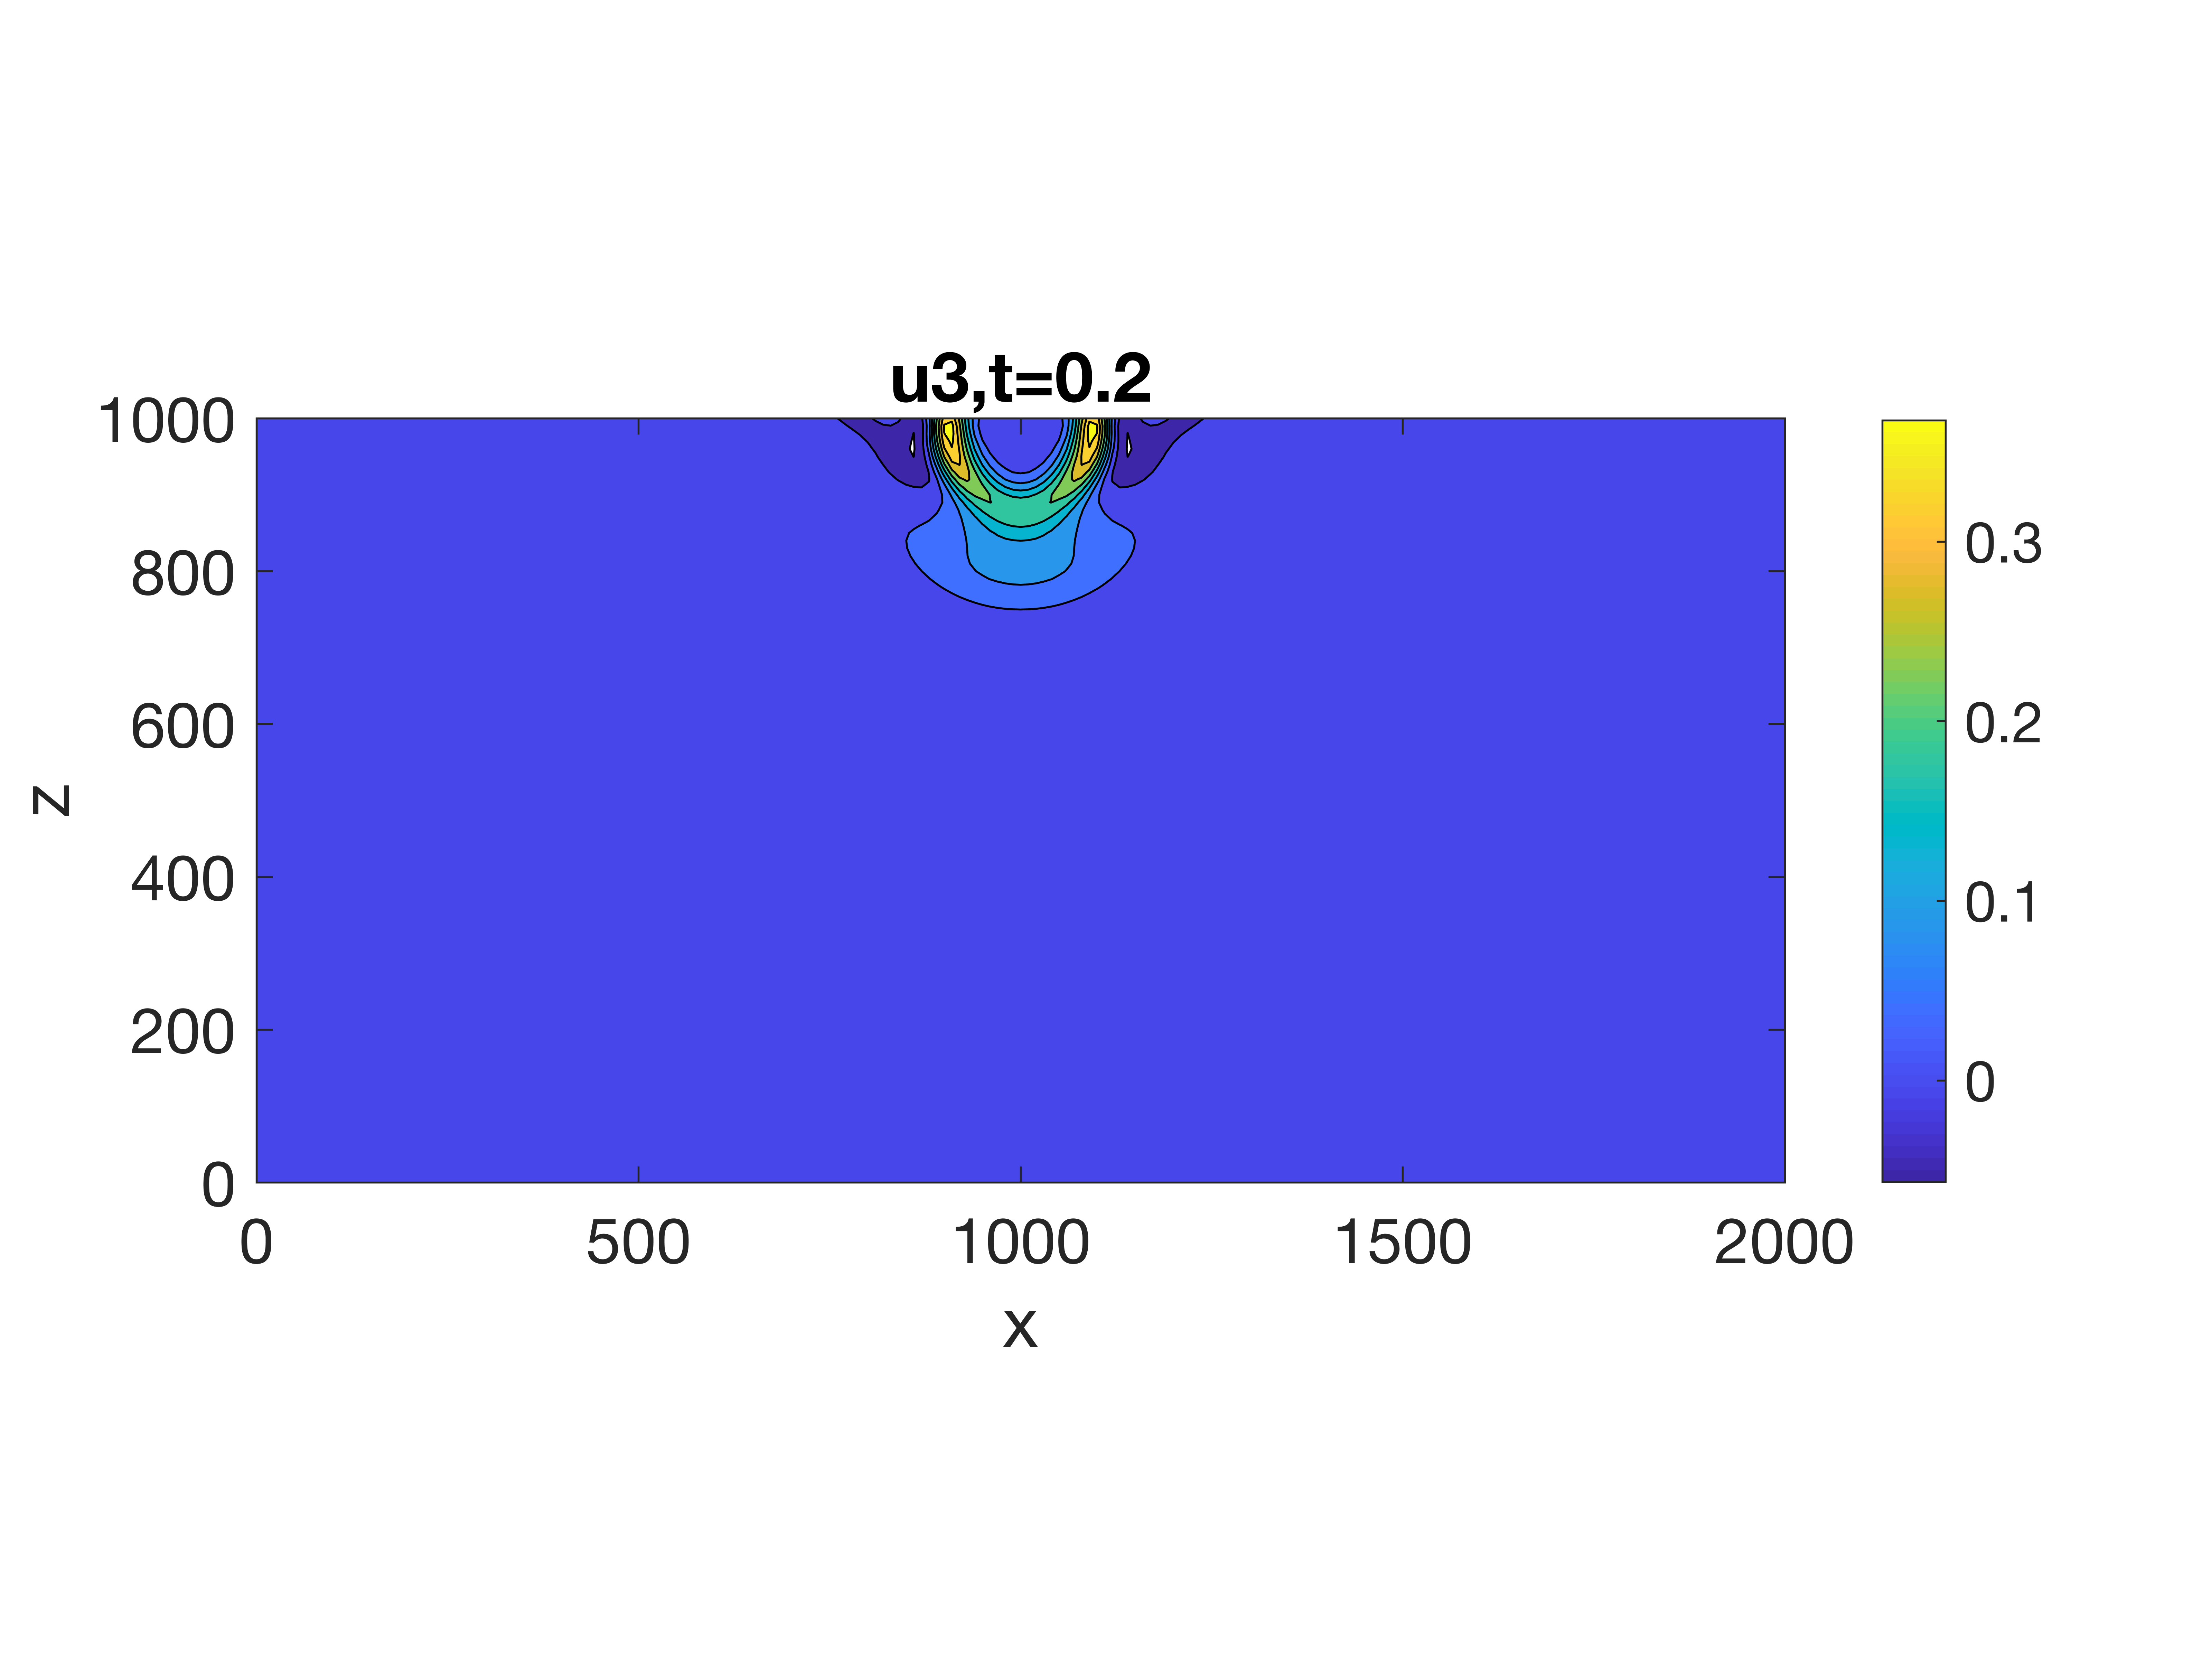
\includegraphics[width=0.4\textwidth,trim={0 2.8cm 0 2.8cm}, clip]{u3_t02_cartesian.png}
	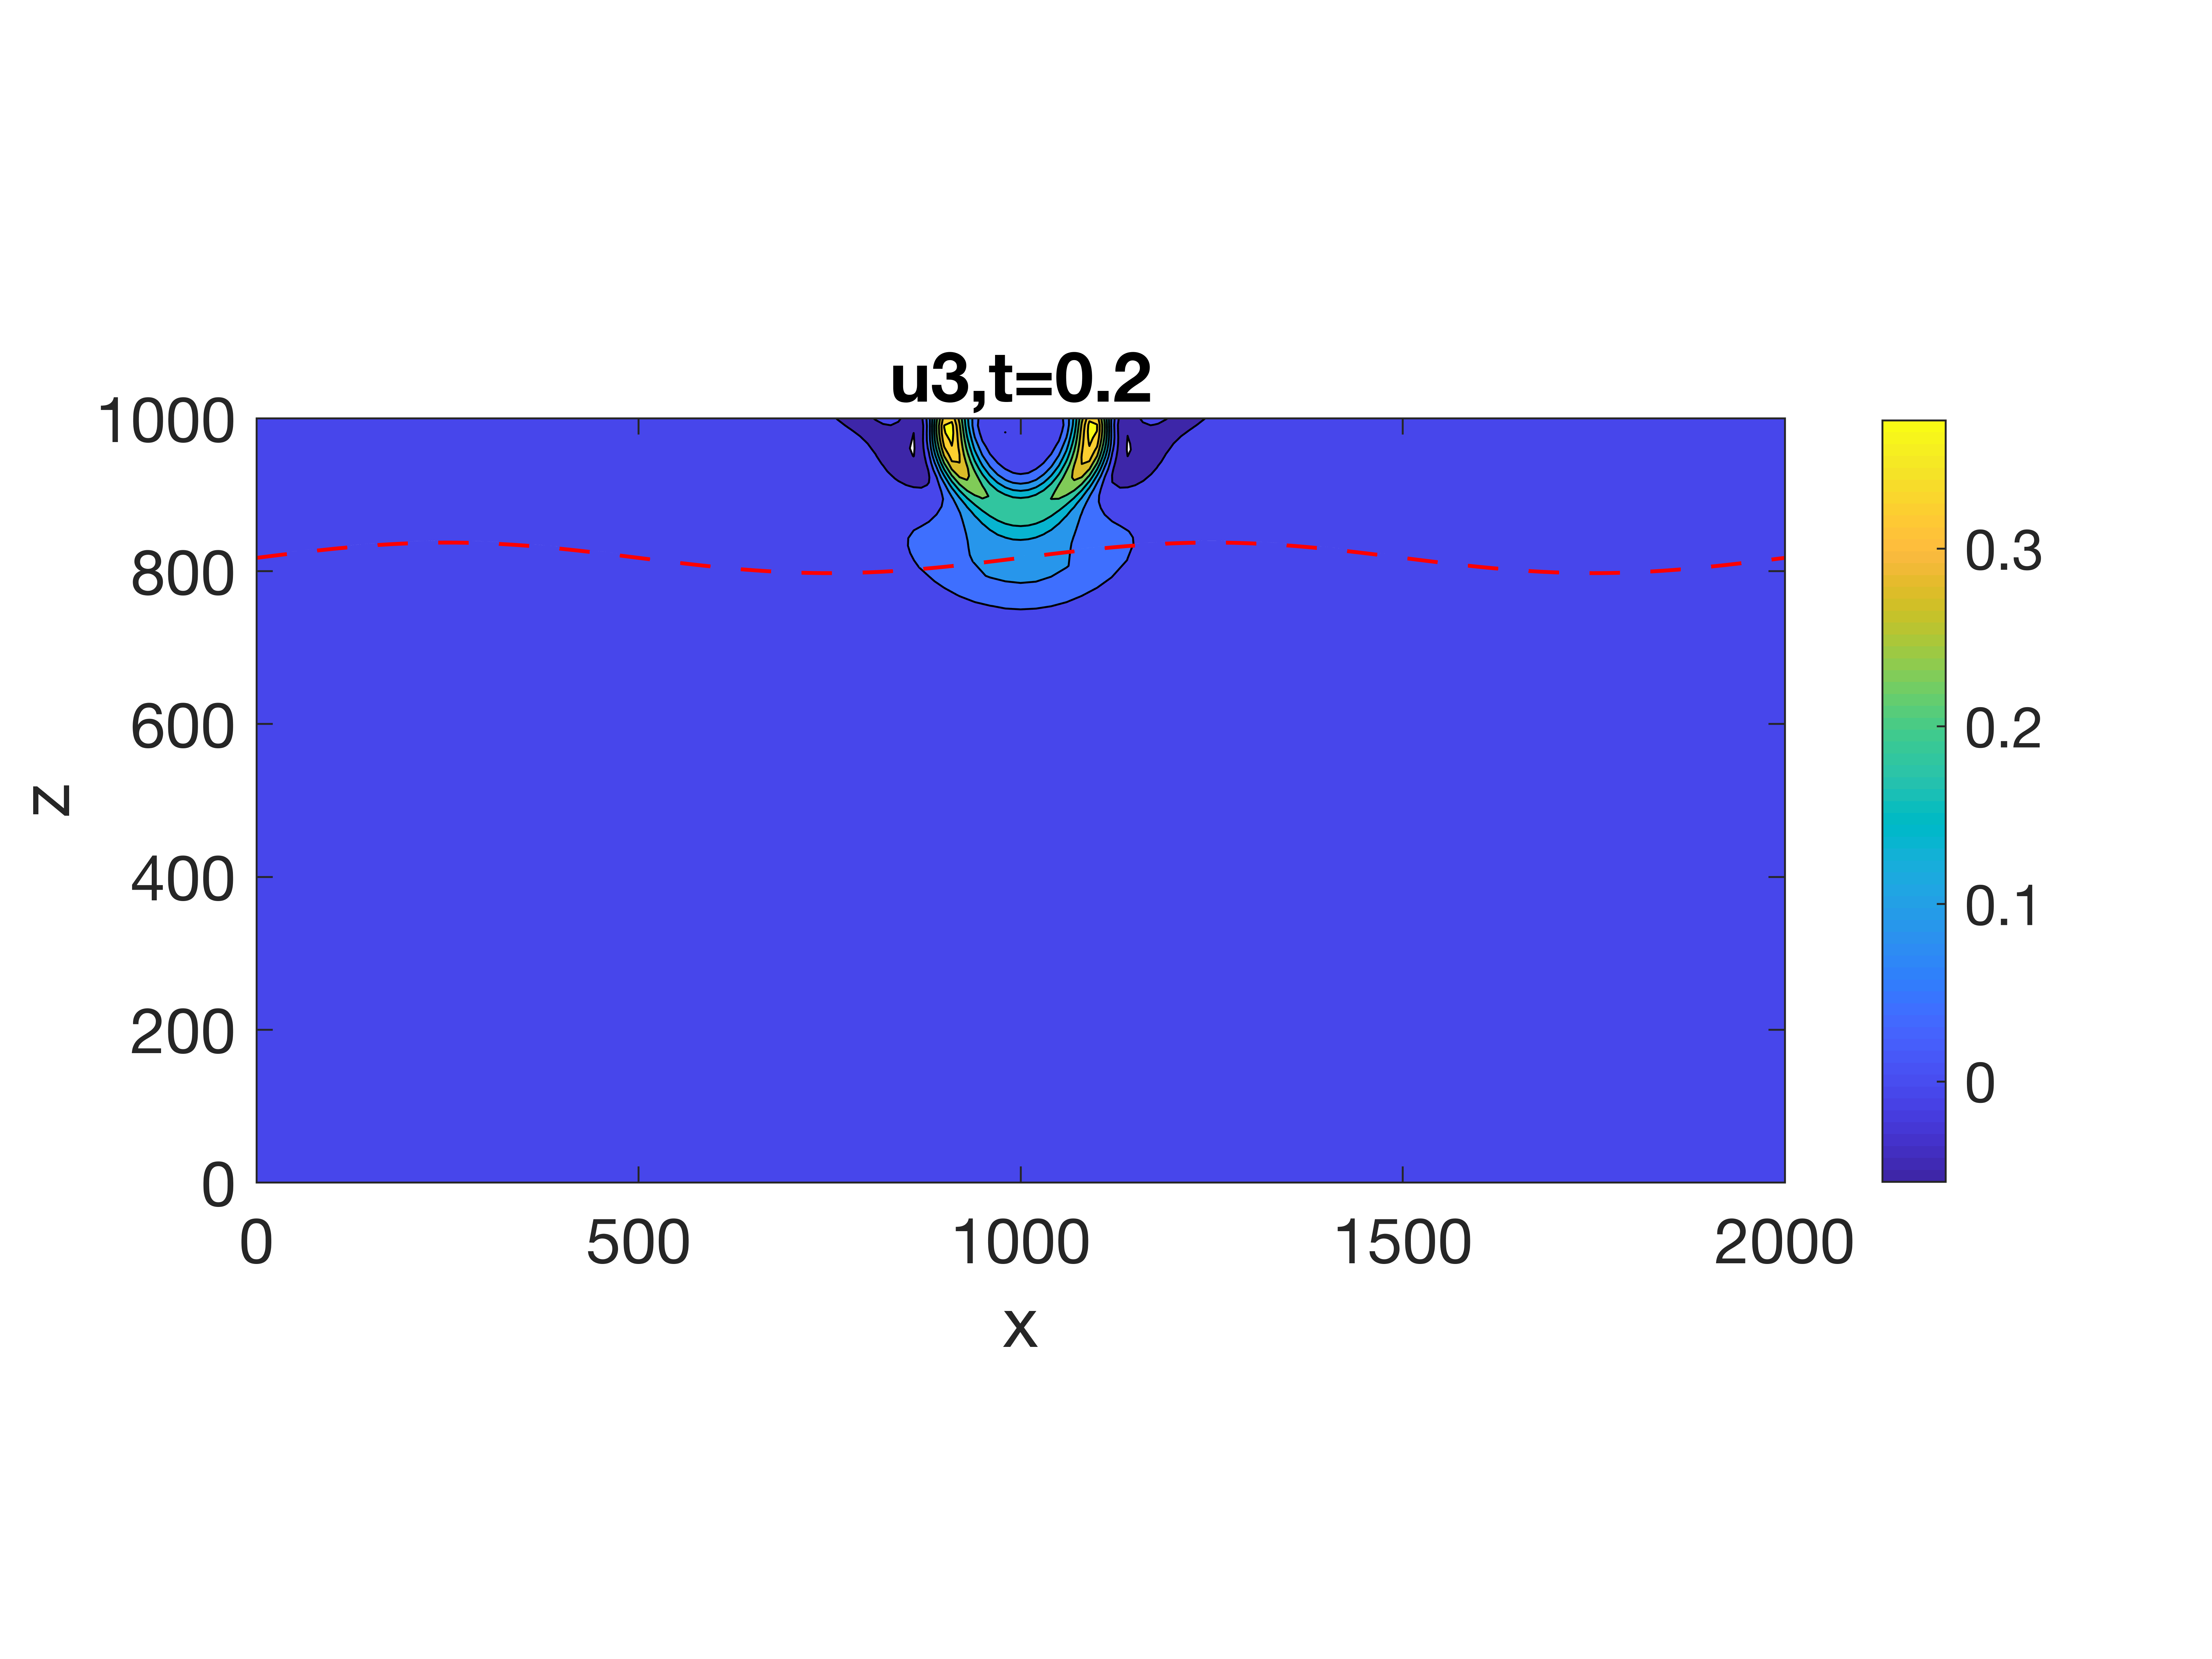
\includegraphics[width=0.4\textwidth,trim={0 2.8cm 0 2.8cm}, clip]{u3_t02_curvi_mr.png}\\
	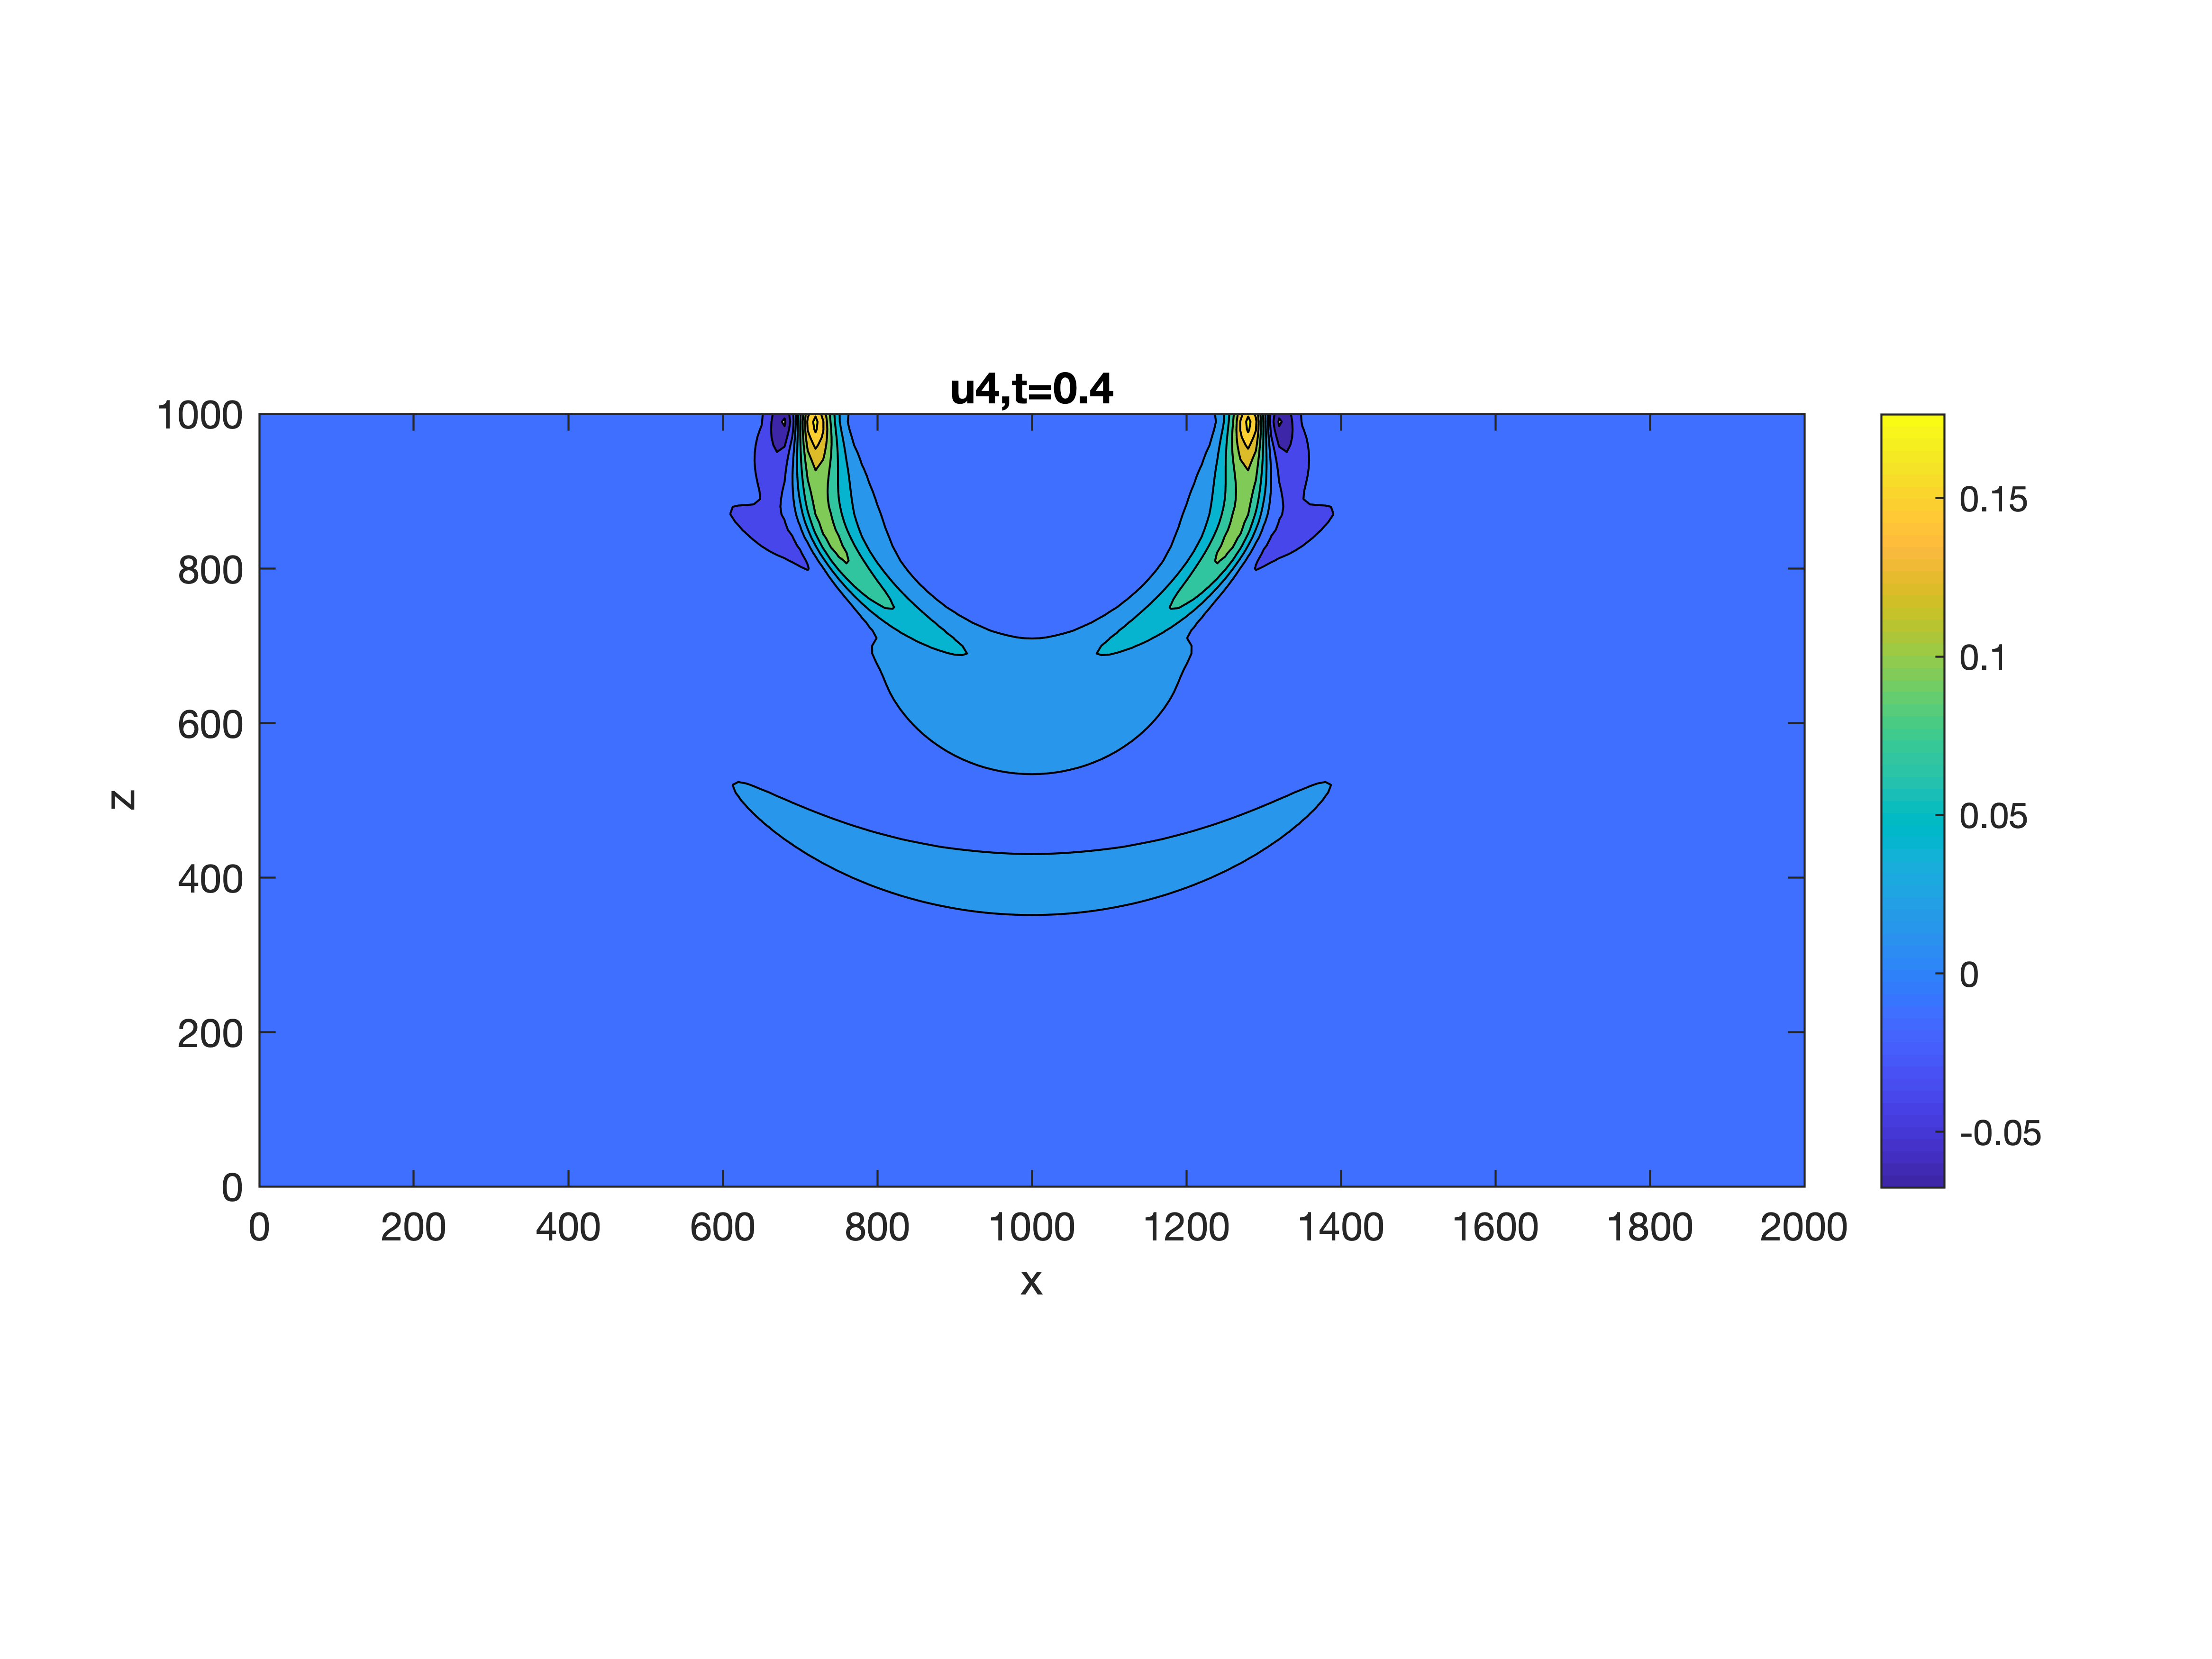
\includegraphics[width=0.4\textwidth,trim={0 2.8cm 0 2.8cm}, clip]{u3_t04_cartesian.png}
	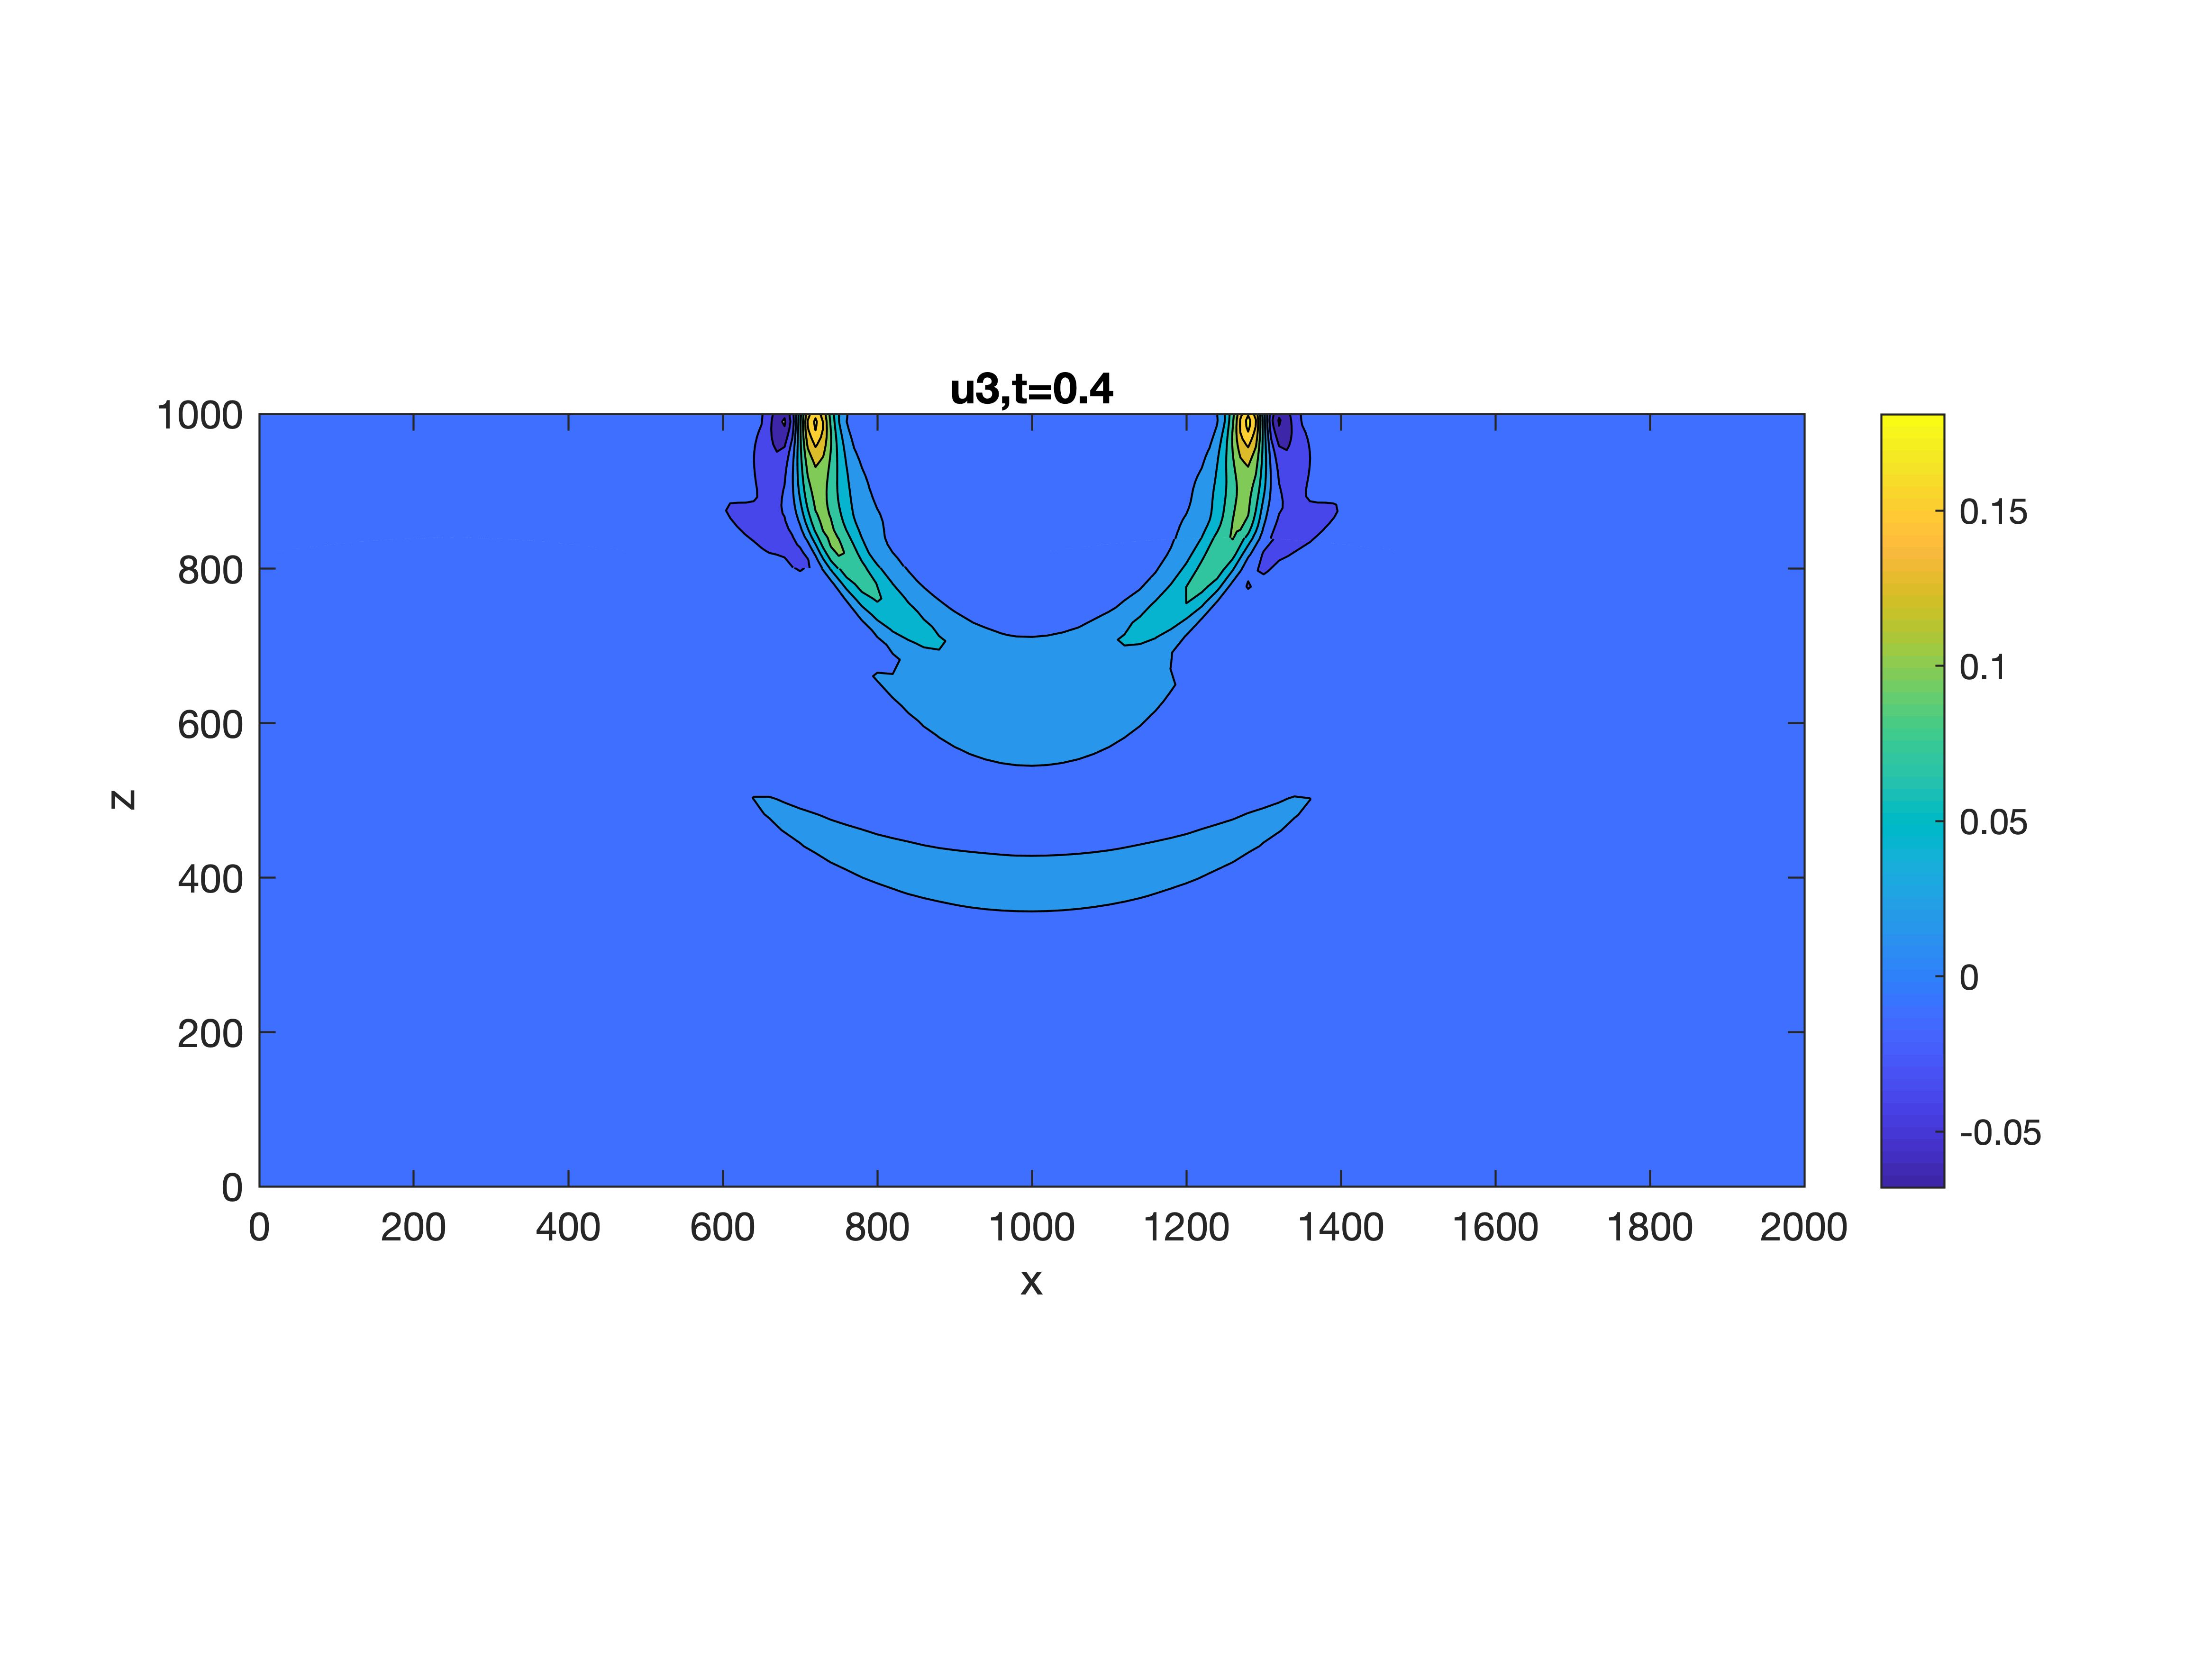
\includegraphics[width=0.4\textwidth,trim={0 2.8cm 0 2.8cm}, clip]{u3_t04_curvi_mr.png}
	\caption{The graph for $u_3$. From left to right are for Cartesian mesh without mesh refinement interface and curvi-linear mesh with mesh refinement interface respectively. From top to bottom are for $t = 0.2$ and $t = 0.4$ respectively.}\label{u3}
\end{figure}
From Figure \ref{u1}, Figure \ref{u2} and Figure \ref{u3}, we observe that there is no significant reflection at the mesh refinement interface.